\chapter{Gas absorption}
 \label{sec:abs_theory}

\graphicspath{{Figs/abs_theory/}}

\starthistory
  2011-07-05 & Revised for ARTS2 by Stefan Buehler.\\
  2001-11-21 & Continuum absorption part written, Thomas Kuhn.\\
  2001-10-05 & Line absorption part written, Nikolay Koulev.\\
\stophistory

% ============================================================================
% TKS definitions for the sections "Continuum Absorption" and 
% "Complete Absorption Models"
%
\def\deni{\rho_{\mbox{\rm i}}}
\def\denl{\rho_{\mbox{\rm l}}}
\def\denli{\rho_{\mbox{\rm l,i}}}
%
\def\imn{{N''}}
\def\ime{\epsilon^{''}_r}
\def\ree{\epsilon^{'}_r}
\def\er{\epsilon_r}
%
\def\bek{\rm b_{\rm 1,k}}
\def\bzk{\rm b_{\rm 2,k}}
\def\bdk{\rm b_{\rm 3,k}}
\def\bvk{\rm b_{\rm 4,k}}
\def\bfk{\rm b_{\rm 5,k}}
\def\bsk{\rm b_{\rm 6,k}}
%
\def\bekp{\rm \widehat{b}_{\rm 1,k}}
\def\bzkp{\rm \widehat{b}_{\rm 2,k}}
\def\bdkp{\rm \widehat{b}_{\rm 3,k}}
\def\bvkp{\rm \widehat{b}_{\rm 4,k}}
\def\bfkp{\rm \widehat{b}_{\rm 5,k}}
\def\bskp{\rm \widehat{b}_{\rm 6,k}}
%
\def\beks{\rm b^*_{\rm 1}}
\def\bzks{\rm b^*_{\rm 2}}
\def\bdks{\rm b^*_{\rm 3}}
\def\bvks{\rm b^*_{\rm 4}}
\def\bfks{\rm b^*_{\rm 5}}
\def\bsks{\rm b^*_{\rm 6}}
%
\def\bekps{\rm \widehat{b^*}_{\rm 1,k}}
\def\bzkps{\rm \widehat{b^*}_{\rm 2,k}}
\def\bdkps{\rm \widehat{b^*}_{\rm 3,k}}
\def\bvkps{\rm \widehat{b^*}_{\rm 4,k}}
\def\bfkps{\rm \widehat{b^*}_{\rm 5,k}}
\def\bskps{\rm \widehat{b^*}_{\rm 6,k}}
%
\def\air{\mbox{air}}
\def\am{\mbox{NH}_3}
\def\hzo{\mbox{H}_2\mbox{O}}
\def\nzo{\mbox{N}_2\mbox{O}}
\def\nz{\mbox{N}_2}
\def\oz{\mbox{O}_2}
\def\co{\mbox{CO}}
\def\coz{\mbox{CO}_2}
\def\clo{\mbox{ClO}}
%
\def\vmroz{VMR_{\mbox{\rm \small O}_{2}}}
%
\def\ptot{P_{\mbox{\rm \small tot}}}
\def\phzo{P_{\mbox{\rm \small H2O}}}
\def\pnz{P_{\mbox{\rm \small N2}}}
\def\poz{P_{\mbox{\rm \small O2}}}
\def\pda{P_{\mbox{\rm \small d}}}
\def\pdair{P_{\mbox{\rm \small air}}}
\def\pan{P_{\mbox{\rm \small air,N2}}}
\def\pcoz{P_{\mbox{\rm \small CO2}}}
%
\def\alphatot{\alpha_{\mbox{\rm \small tot}}} 
\def\alphal{\alpha_{\ell}} 
\def\alphac{\alpha_{\mbox{\small c}}}
\def\alphacs{\alpha_{\mbox{\rm \small c,s}}} 
\def\alphacf{\alpha_{\mbox{\rm \small c,f}}}
%
\def\alphampmotot{\alpha^{\mbox{\rm \small MPM87}}_{\mbox{\small tot}}} 
\def\alphampmmtot{\alpha^{\mbox{\rm \small MPM89}}_{\mbox{\small tot}}} 
\def\alphampmntot{\alpha^{\mbox{\rm \small MPM93}}_{\mbox{\small tot}}} 
\def\alphapwrtot{\alpha^{\mbox{\rm \small R98}}_{\mbox{\small tot}}} 
\def\alphacptot{\alpha^{\mbox{\rm \small CP98}}_{\mbox{\small tot}}} 
%
\def\alphampmol{\alpha^{\mbox{\rm \small MPM87}}_{\mbox{\small $\ell$}}} 
\def\alphampmml{\alpha^{\mbox{\rm \small MPM89}}_{\mbox{\small $\ell$}}} 
\def\alphampmnl{\alpha^{\mbox{\rm \small MPM93}}_{\mbox{\small $\ell$}}} 
\def\alphampml{\alpha^{\mbox{\rm \small MPM}}_{\mbox{\small $\ell$}}} 
\def\alphapwrl{\alpha^{\mbox{\rm \small R98}}_{\mbox{\small $\ell$}}} 
\def\alphacpl{\alpha^{\mbox{\rm \small CP98}}_{\mbox{\small $\ell$}}} 
%
\def\alphampmoc{\alpha^{\mbox{\rm \small MPM87}}_{\rm c}} 
\def\alphampmmc{\alpha^{\mbox{\rm \small MPM89}}_{\rm c}} 
\def\alphampmnc{\alpha^{\mbox{\rm \small MPM93}}_{\rm c}} 
\def\alphapwrc{\alpha^{\mbox{\rm \small R98}}_{\rm c}} 
\def\alphacpc{\alpha^{\mbox{\rm \small CP98}}_{\rm c}} 
%
\def\gamk{\gamma_{\mbox{\rm \small k}}}
\def\gamc{\gamma_{\mbox{\rm \small c}}}
%
\def\ws{w_{\mbox{\rm \small s,k}}}
\def\xs{x_{\mbox{\rm \small s,k}}}
\def\wf{w_{\mbox{\rm \small f,k}}}
\def\xf{x_{\mbox{\rm \small f,k}}}
%
\def\wn{\bar{\nu}}
\def\nucc{\nu_{\mbox{\rm \small c}}}
\def\nucut{\nu_{\mbox{\rm \small cutoff}}}
\def\nuo{\nu_{\mbox{\rm \small 0}}}
\def\nuk{\nu_{\mbox{\rm \small k}}}
%
\def\shape{F(\nu,\nuk)}
\def\shapec{F_{c}(\nu,\nuk)}
\def\shapefp{f_{c}(\nu,+\nuk)}
\def\shapefm{f_{c}(\nu,-\nuk)}
\def\shapefpm{f_{c}(\nu,\pm\nuk)}
\def\inten{S_{\mbox{\rm \small k}}(T)}
\def\inteno{S_{\mbox{\rm \small k}}(300\,K)}
\def\intencp{S_{\mbox{\rm \small 0}}(T)}
%
\def\cx{C_{\mbox{\rm \small x}}}
\def\cs{C_{\mbox{\rm \small H}_{2}\mbox{\rm \small O}}} 
\def\cf{C_{\mbox{\rm N}_{2}}} 
\def\cxo{C^{\mbox{\rm o}}_{\mbox{\rm \small X}}} 
\def\cso{C^{\mbox{\rm o}}_{\mbox{\rm \small H}_{2}\mbox{\rm \small O}}} 
\def\cfo{C^{\mbox{\rm o}}_{\mbox{\rm \small N}_{2}}} 
\def\cao{C^{\mbox{\rm o}}_{\mbox{\rm \small air}}}
\def\cdo{C^{\mbox{\rm o}}_{\mbox{\rm \small d}}}
\def\xx{{\rm n}_{\mbox{\rm \small  x}}} 
\def\xs{{\rm n}_{\mbox{\rm \small  s}}} 
\def\xf{{\rm n}_{\mbox{\rm \small  f}}} 
\def\xd{{\rm n}_{\mbox{\rm \small  d}}}
%
% ============================================================================

This chapter contains theoretical background and scientific details
for gas absorption calculations in ARTS. A more practical overview,
with focus on how to set up calculations, is given in \user, Chapter
\ref{U-sec:absorption}.

Gas absorption generally consists of a superposition of spectral lines
and continua.  Depending on the gas species, the continua either have
a real physical meaning, or they are more or less empirical
corrections for deficits in the explicit line-by-line calculation.  In
the latter case the magnitude of the continuum term will depend
strongly on the exact setup of the line-by-line calculation.
Combining continua and line-by-line calculation therefore requires
expertise.

This chapter is structured in three main parts: Line absorption,
continuum absorption, and complete absorption models. It should be
noted that the three topics are tightly related. In particular,
complete absorption models will normally include a line part and a
continuum part. Some absorption models, notably those by Rosenkranz
and Liebe will show up under both continua and complete absorption
models. The continuum section then treats specifically the continuum
parameterization of these model, the complete absorption model section
puts more focus on the line part and the model as a whole.

Each of the main parts first introduces the theoretical background to the topic,
then presents aspects of the specific implementation in ARTS.
                                          

% ================================================================================
% The following section was originally written by Nikolay Koulev, iup
% Bremen, nkoulev@uni-bremen.de
% Edit in 2011 by Stefan Buehler
% ================================================================================

\section{Line absorption}
%-----------------------
\label{sec:abs_theory:line_absorption}

\subsection{Theoretical background}
 
We will introduce here the main concepts concerning line
absorption. The aim is to give some overview and show some key
equations, not to give a full treatment of the theory. To really
understand line absorption, you should refer to one of the cited
books, or some other book on spectroscopy.

\subsubsection{Basic expressions} 

An absorption line is described by the corresponding 
absorption coefficient as a function of frequency $\alpha(\nu)$, which
can be written as \citep{goodyandyung:89}:
\begin{equation}\label{eq:abs_coeff}
  \alpha(\nu)=nS(T)F(\nu)
\end{equation} 
where $S(T)$ is called the line strength, $T$ is the temperature,
$F(\nu)$ is called the line shape function, and
$n$ is the number density of the absorber. The line shape
function is normalized as:
\begin{equation}\label{eq:abs_theory:line_shape_norm}
  \int F(\nu)d\nu=1
\end{equation}

The values of $S(T)$ at reference temperature $T_0$ are contained in
spectroscopic databases (more on this below). The conversion to
different temperatures is done by
\begin{equation}\label{eq:abs_theory:line_intensity}
  S(T)=S(T_0)~\frac{Q(T_0)}{Q(T)}~\frac{e^{-E_f/(kT)}
    - e^{-E_i/(kT)}}{e^{-E_f/(kT_0)} - e^{-E_i/(kT_0)}}
\end{equation}
given the energies $E_f$ and $E_i$ of the two levels between which the
transition occurs as well as the partition function  $Q(T)$ \citep{rothman:98}.
The databases contain the lower state energy $E_l$ tabulated along with
the $S$ and the transition frequency $\nu$, so that the upper state
energy can be computed by $E_u$=$E_l$+h$\nu$. Partition functions for
the different molecular species are commonly available along with the
spectroscopic databases, given in the form of tabulated values for a set
temperatures (e.g., for JPL catalogue) or through some computer code (e.g.,
the TIPS program coming with the HITRAN catalogue). As absorption is additive,
the total absorption coefficient is derived by adding up the absorption
contributions of all spectral lines of all molecular species.

The following subsections discuss common descriptions of the line shape
function, present partition functions and their calculation formalism more in
depth, and introduce the Zeeman effect.


\subsubsection{Line shape functions} 
\label{sec:abs_theory:shape}

So far, there exists no complete analytical function that accurately
describes the line shape in all atmospheric conditions and for all
frequencies. But for most cases very accurate approximations are
available. Which approximation is appropriate depends mostly on the
atmospheric pressure, and on whether the frequencies of interest are
close to the line center, or far out in the line wing.

There are three phenomena which contribute to the line shape. These
are, in increasing order of importance, the finite lifetime of an
excited state in an isolated molecule, the thermal movement of the gas
molecules, and their collisions with each other. They result in
corresponding effects to the line shape: natural broadening, Doppler,
and pressure broadening. Of these, the first one is completely
negligible compared to the other two for typical atmospheric
conditions. Nevertheless, we will pay a special attention to the
natural broadening because its implications are of a conceptual
importance for the broadening processes.

The spectral line shape can be derived in the case of natural
broadening from basic physical considerations and a well-known Fourier
transform theorem from the time to the frequency domain \citep{thorne:99}. If we
consider classically the spontaneous decay of the excited state of a
two-level system in the absence of external radiation, then the population
$n$ of the upper level decreases according to
\begin{equation}\label{eq:abs_theory:spon_decay_diff}
  \frac{dn(t)}{dt} = -A\,n(t)
\end{equation}
where $A$ is Einstein A coefficient. This equation can also be
interpreted as the rate of the spontaneously emitted photons because
of decay. The integral form of this relation is 
\begin{equation}\label{eq:abs_theory:spon_decay_exp}
  n(t)=n(0)~e^{-At}=n(0)e^{-t/\tau}
\end{equation}
where $ \tau$ is the mean lifetime of the excited state. Thus, the
number of spontaneously emitted photons and in this way the flux of
the emitted radiation then will be proportional to $n$. Therefore we
can write for the flux $L$ that
\begin{equation}\label{eq:abs_theory:flux}
  L(t)=L(0)~e^{-t/ \tau}=L(0)~e^{-\gamma t}
\end{equation}
By the afore mentioned theorem, multiplying in the time domain by
$e^{-\gamma t}$ is equivalent to convolving in the frequency domain
with a function $1/[\nu^2 - (\gamma/4\pi)^2]$. Accordingly, the line
profile of a spectral line at frequency $ \nu_0$ as a normalized
line shape function will be, as defined in \citet{thorne:99},
\begin{equation}\label{eq:abs_theory:natural_lorentz}
  F(\nu)=\frac{1}{\pi}\frac{\gamma/4\pi}{(\nu - \nu_0)^2 + (\gamma/4\pi)^2}
\end{equation}
This gives a bell-shaped profile and the function itself is called
Lorentzian. The dependence on the position of the line is apparent
through $\nu_0$, that is why some authors prefer to denote the
function by $F(\nu,\nu_0)$.  The result is important because of two
major reasons.  Firstly, without the natural broadening the line would
be the delta function $\delta (\nu - \nu_o)$, as pointed out in
\citet{bernath:95}. So the spontaneous decay of the excited state is
responsible for the finite width and the certain shape of the
line shape function. Secondly, the Lorentzian type of function comes
significantly into play when explaining some of the other broadening
effects or the complete picture of the broadened line \citep{thorne:99}.

The second effect, Doppler broadening, is important for the upper
stratosphere and mesosphere for microwave frequencies. The line shape
follows the velocity distribution of the particles. Under the conditions
of thermodynamic equilibrium, we have  a probability distribution for
the relative velocity $u$ between the gas molecule and the observer 
of Maxwell type 
\begin{equation}\label{eq:abs_theory:maxwell_distribution1}
  p(u)=\sqrt{\frac{m}{2\pi kT}}~~exp~\left[-\frac{mu^2}{2kT}\right]
\end{equation}
where $m$ is the mass of the molecule. Using then the formula for the
Doppler shift for the non-relativistic region    $\nu$- $\nu_0$ =
$\nu_0$$u$ / $c$ , one can easily derive the line shape function \citep{bernath:95}, 
\begin{equation}
 F_D(\nu)=\frac{1}{\gamma_D\sqrt{\pi}}~~exp~\left[-\left(\frac{\nu - \nu_0}{\gamma_D}\right)^2\right]
\end{equation}
where the quantity $\gamma_D$ is called Doppler line width and equals
\begin{equation}
 \gamma_D=\frac{\nu}{c}\sqrt{\frac{2kT}{m}}
\end{equation}
In contrast to the line shape function for the natural
broadening, the Doppler broadening leads to a Gaussian
line shape function $F(\nu)$. The Doppler line width $\gamma_D$ is so
defined that it is equal to the half width at half of the maximum
(HWWM) of the line shape function. A similar notation is used
for all other width parameters $\gamma_{xy}$ below.

The third broadening mechanism is pressure broadening.  It is the most
complicated broadening mechanism, and still subject to theoretical and
experimental research. So far, there is no way to derive the exact
shape of a pressure-broadened line from first principles, at least not
for the far wing region. The various approximations, which are
therefore used, are immanently limited to the certain line regions
they deal with.  The most popular among these approximations is the
{\it{impact approximation}} which postulates that the duration of the
collisions of the gas particles is very small compared to the average
time between the collisions.  Due to the Fourier-pair relationship
between time and frequency, the line shape that follows from the
impact approximation can only be expected to be accurate near the line
center, not in the far wings of the line.

Lorentz was the first to achieve a result exploiting the impact
approximation, the Lorentz line shape function:
\begin{equation}\label{eq:abs_theory:pressure_lorentz}
 F_L(\nu)=\frac{\gamma_L}{\pi}\frac{1}{(\nu-\nu_0)^2+\gamma_L^2}
\end{equation}
where $\gamma_L$ is the Lorentz line width \citep{thorne:99}. As one
can see, the result Eq.\,\ref{eq:abs_theory:pressure_lorentz} is pretty similar to
Eq.\,\ref{eq:abs_theory:natural_lorentz} but the specific line parameters $\gamma$
and $\gamma_L$ make them differ significantly in the corresponding
frequency regions of interest. For atmospheric pressures $\gamma_L$ is
much greater and because of that, of experimental
significance in contrast to $\gamma$.\\
Elaborating the model of Lorentz, van Vleck and Weisskopf made a
correction to it \citep{vanvleck:45},particularly for the microwave
region:
\begin{equation}\label{eq:abs_theory:vvw}
 F_{VVW} (\nu)=\left(\frac{\nu}{\nu_0}\right)^2\frac{\gamma_L}{\pi}
 \left[\frac{1}{(\nu-\nu_0)^2+\gamma_L^2}+\frac{1}{(\nu+\nu_0)^2+\gamma_L^2}\right]
\end{equation}
which can be reduced to a Lorentzian for $(\nu-\nu_0) << \nu_0$ and $0
<< \nu_0$. Except for the additional factor $(\nu/\nu_0)^2$ ,
$F_{VVW}$ can be regarded as the sum of two $F_L$
lines, one with its center frequency at $\nu_0$, the other at
$-\nu_o$.

The van Vleck and Huber lineshape \citep{vanvleckhuber:77} is similar
to Eq.\,\ref{eq:abs_theory:vvw}, except for the factor $(\nu/\nu_0)^2$ which is
replaced by $(\nu * \tanh(h*\nu/(2kT)))/(\nu_0 *
\tanh(h*\nu_0/(2kT)))$, with $k$ the Boltzmann constant, $h$ the Planck
constant, and $T$ the atmospheric temperature (the denominator is
actually a consequence of the line strength definition in the
spectroscopic catalogs). The lineshape Eq.\,\ref{eq:abs_theory:vvw} with this
factor can be used for the entire frequency range, since
the microwave approximation: $\tanh(x) = x$, that leads to the factor
$(\nu/\nu_0)^2$, is not made.

The combined picture of a simultaneously Doppler and pressure
broadened line is the next step of the approximations development. The
line shape function has to approximated in this case by the Voigt line shape
function 
\begin{equation}\label{eq:abs_theory:voigt}
 F_{Voigt}(\nu,\nu_0)= \int F_L(\nu,\nu')~F_D(\nu',\nu_0)~d\nu'
\end{equation}
though there's no strict justification for its use - the two processes
are assumed to act independently, which in reality is not the
fact. Regardless of this flaw, it is the only way up to now to model
the combination of the broadening processes. The integral in Eq.\,\ref{eq:abs_theory:voigt}
can not be computed analytically, so certain approximation algorithms
must be used.


Another possibility would be the combination of the last two equations
Eq.\,\ref{eq:abs_theory:vvw} and Eq.\,\ref{eq:abs_theory:voigt}. The respective result then will be 
\begin{equation}\label{eq:abs_theory:voigt_mirror}
 F_S=\left(\frac{\nu}{\nu_0}\right)^2~[F_{Voigt}(\nu,\nu_0)+F_{Voigt}(\nu,-\nu_0)]
\end{equation}
The advantage of such a model is that it behaves like a van
Vleck-Weisskopf line shape function in the high pressure limit and
like a Voigt one in the low pressure limit. There is one important
caveat to the equation Eq.\,\ref{eq:abs_theory:voigt_mirror}: it has to be made sure
that the algorithm that is used to compute the Voigt function really
produces a Lorentz line in the high pressure limit. Another point of
significance is the demand that the model yields meaningful results
far from the line center, since the line center from the ``mirror''
line at -$\nu_0$ is situated approximately 2$\nu_0$ away from the
frequency $\nu_0$ of computation. We explicitly verified that the
algorithms of \citet{Drayson:76}, \citet{Oliveiro:77}, and
\citet{kuntz:99} satisfy both requirements, while this was found to be
not true for some other algorithms commonly used for Voigt-shape
computation. In particular, it is not true for the Hui-Armstrong-Wray
Formula, as defined in \citet{hui:78} and in Equation 2.60 of
\citet{pwr:93}. Provided the condition above is fulfilled, the $F_S$
line shape gives a smooth transition from high tropospheric pressures
to low stratospheric ones, and should be valid near the line centers
throughout the microwave region. With a Van Vleck / Huber forefactor
instead of the Van Vleck / Weisskopf forefactor, it should be valid
throughout the thermal infrared spectral range, but there the mirror
line at negative frequency is negligible anyway, because it is so far
away.


\subsubsection{Partition functions}

Partition functions are needed to compute the temperature dependence
of the line intensities (Equation \ref{eq:abs_theory:line_intensity} on
page \pageref{eq:abs_theory:line_intensity}).  They are related to the
molecular energy states and their statistical distribution during the
radiation process.

In any case of spectroscopic interest the free molecules of a gas are
not optically thick at all frequencies, so the radiation energy is not
represented by blackbody radiation. The most common assumption made,
which is sufficient in the case of tropospheric and low stratospheric
research, is the {\textit{local thermodynamic equilibrium}\nocorr} or
{\textit{LTE}\nocorr}. According to it, it's possible to find a common temperature,
which may vary from place to place, that fits the Boltzmann energy
population distribution and the Maxwell velocities distribution.
This practically means, that under $LTE$ the collisional processes
must be of greater importance than radiative ones. In other words,
an excited state must have a higher probability of de-excitation by
collision than by spontaneous radiation. This is the important
factor which makes natural broadening differ quantitatively so much
from the pressure (collisional) one, though both are described
qualitatively almost identically by Lorentzian line shape
functions.

According to the Maxwell-Boltzmann distribution law, in $LTE$ the total number
of gas particles $N_n$  in a state $E_n$ is given by 
\begin{equation}\label{eq:abs_theory:maxwell_distribution2}
 N_n=N_0\frac{g_n}{g_0}e^{-E_n/kT}
\end{equation}
where $N_0$ is particle number in the ground state, and $g_n$, $g_o$
are the statistical weights (degeneracies) of the $n-$state and the
ground state \citep{gordyandcook:70}. Thus the total particle number $N$ is given by
\begin{equation}\label{eq:abs_theory:total_part_number}
 N=\frac{N_0}{g_0}\sum_{n=0}^\infty g_n~e^{-E_n/kT}=\frac{N_0}{g_0}~Q(T)
\end{equation}
The quantity $Q(T)$ is the {\it{partition function}\nocorr} of the
gas, which generally speaking describes the energy states distribution
of the gas particles. 

The partition function for a perfect gas molecule can be represented
by the product of the {\it{translational}\nocorr} and the
{\it{internal}\nocorr} partition functions, as defined in \citet{herzberg:45},
\begin{equation}\label{eq:abs_theory:partition_f_general}
 Q  =  Q_{tr}~Q_{int}
\end{equation}
bearing in mind that the respective energies, translational and
internal, are independent of each other. The first quantity $Q_{tr}$ accounts
for the distribution of the translational energy of the gas particles
- it takes into account that the translational velocities of the
particles fulfill the Maxwell distribution. However, for Equation
\ref{eq:abs_theory:line_intensity}, the quantity we are interested in
is the {\it{internal}\nocorr} partition function (or the {\it{total internal
partition function}\nocorr}) because the transitions between the discrete
internal energy states are responsible for the absorption or emittance
of radiation. Accordingly $Q_{int}$ describes the distribution of energy among
the internal energy states of the gas particles.

The internal partition function for free gaseous molecules is a
function of the electronic, the vibrational, the rotational, and the
nuclear spin states. An approximation is used in
\citet{gordyandcook:70} in order to display the individual
contributions explicitly
\begin{equation}\label{eq:abs_theory:int_partition}
 Q_{int}=Q_e~Q_v~Q_r~Q_n
\end{equation}
and thus the interaction between these various states is neglected.
For practically all polyatomic molecules the excited electronic states
are entirely negligible to those of the ground states, i.e. $Q_e=1$ .
Only for the very few polyatomic molecules with a multiplet ground
state ($NO_2$ , $ClO_2$ , and free radicals) the
electronic contribution has to be considered.\\
If we neglect the anharmonicities, the vibrational partition function,
with vibrational energy levels measured with respect to the ground
state for the {\it harmonic oscillator}, is according to \citet{herzberg:45}
\begin{equation}\label{eq:abs_theory:vib_partition}
 Q_v=\left(\sum_{\nu_1}e^{-\nu_1 h\omega_1/kT}\right)\left(\sum_{\nu_2}e^{-\nu_2 h\omega_2/kT}\right)...
\end{equation}
where $\nu_1$, $\nu_2$,..., the vibrational quantum numbers, can each
have the values 0,1,2,... and $\omega_1$, $\omega_2$,..are the
frequencies of the fundamental modes of vibration. The summation is
taken over all values of $\nu_1$, $\nu_2$,..., and each fundamental
mode is counted separately. This result is valid for non-degenerate
vibrations. If we use the simple expression for geometric progression
\begin{equation}\label{eq:abs_theory:geom_progression}
 \sum_{\nu_i}e^{-\nu_i h\omega_i/kT}=\frac{1}{1-e^{h\omega_i/kT}}
\end{equation}
and the degeneracies $d_1$, $d_2$,... of the fundamental modes, we get
finally for the vibrational partition function
\begin{equation}\label{eq:abs_theory:vib_partition_fin}
Q_v=\left(1-e^{h\omega_1/kT}\right)^{-d_1}\left(1-e^{h\omega_2/kT}\right)^{-d_2}...
\end{equation}

The rotational partition function looks differently for the different
symmetry types of molecules.
For diatomic and linear  polyatomic molecules with no center of
symmetry the corresponding expression is, as defined in \citet{gordyandcook:70}
\begin{eqnarray}\label{eq:abs_theory:rot_partition}
Q_r & = & \sum_{J=0}^\infty (2J+1)e^{-hBJ(J+1)/kT}\nonumber\\
   & = & \frac{kT}{hB}+\frac{1}{3}+\frac{1}{15}\frac{hB}{kT}+\frac{4}{315}\left(\frac{hB}{kT}\right)^2+...\nonumber\\
   & \cong & \frac{kT}{hB}
\end{eqnarray}
For {\it{ rigid symmetric-}}, {\it{asymmetric-}}, and {\it{spherical}} top molecules there are also
other factors to be taken into consideration, such as the
spatial structure of the molecules, nuclear spin, inversion and
internal rotation. The general expression in the case of a 
{\it{ rigid symmetric-}} top molecule according to \citet{herzberg:45}
is
\begin{equation}\label{eq:abs_theory:rot_partition_symtop}
Q_r  =  \frac{1}{\sigma}\sum_{J=0}^\infty \sum_{K=-J}^{J}(2J+1)~e^{-h[BJ(J+1)+(A-B)K^2]/kT}
\end{equation}
where $\sigma$ is a measure of the degree of symmetry. The usual
symmetric top has $C_3$ or $C_{3\nu}$ symmetry, therefore $\sigma$ = 3. To a good
approximation, the summation above can expressed as in \citet{gordyandcook:70}
\begin{equation}\label{eq:abs_theory:rot_partition_top_appro}
Q_r  = 
\frac{1}{\sigma}\left[\left(\frac{\pi}{B^2A}\right)\left(\frac{kT}{h}\right)^3\right]^{1/2}=
\frac{5.34\times 10^6}{\sigma}\left(\frac{T^3}{B^{2}A}\right)^{1/2}
\end{equation}
For an  {\it{asymmetric}} top the formula would then be 
\begin{equation}\label{eq:abs_theory:rot_partition_asymtop}
Q_r = \frac{5.34\times 10^6}{\sigma}\left(\frac{T^3}{ABC}\right)^{1/2}
\end{equation}
and for a {\it{spherical}} top, using the current notation of
\citet{gordyandcook:70} in the respective expression in \citet{herzberg:45},
\begin{equation}\label{eq:abs_theory:rot_partition_sphetop}
Q_r = \frac{5.34\times 10^6}{\sigma}\left(\frac{T^3}{A^3}\right)^{1/2}
\end{equation}

\subsubsection{The Zeeman Effect for O$_2$}
Gases with an inherent magnetic dipole placed in an external magnetic field show a special kind of transition. This is known as the Zeeman effect, which polarizes the radiation and results in several shifted peaks per line. In essence it increases the number of lines, which means that we can treat each peak as a separate absorption line of a relatively different strength and with a shifted central frequency. Of course, we must also consider the polarization effect (which is mathematically sound to do with rotating matrices in Stokes parameterization).

\begin{figure}[ht!]
 \centering
 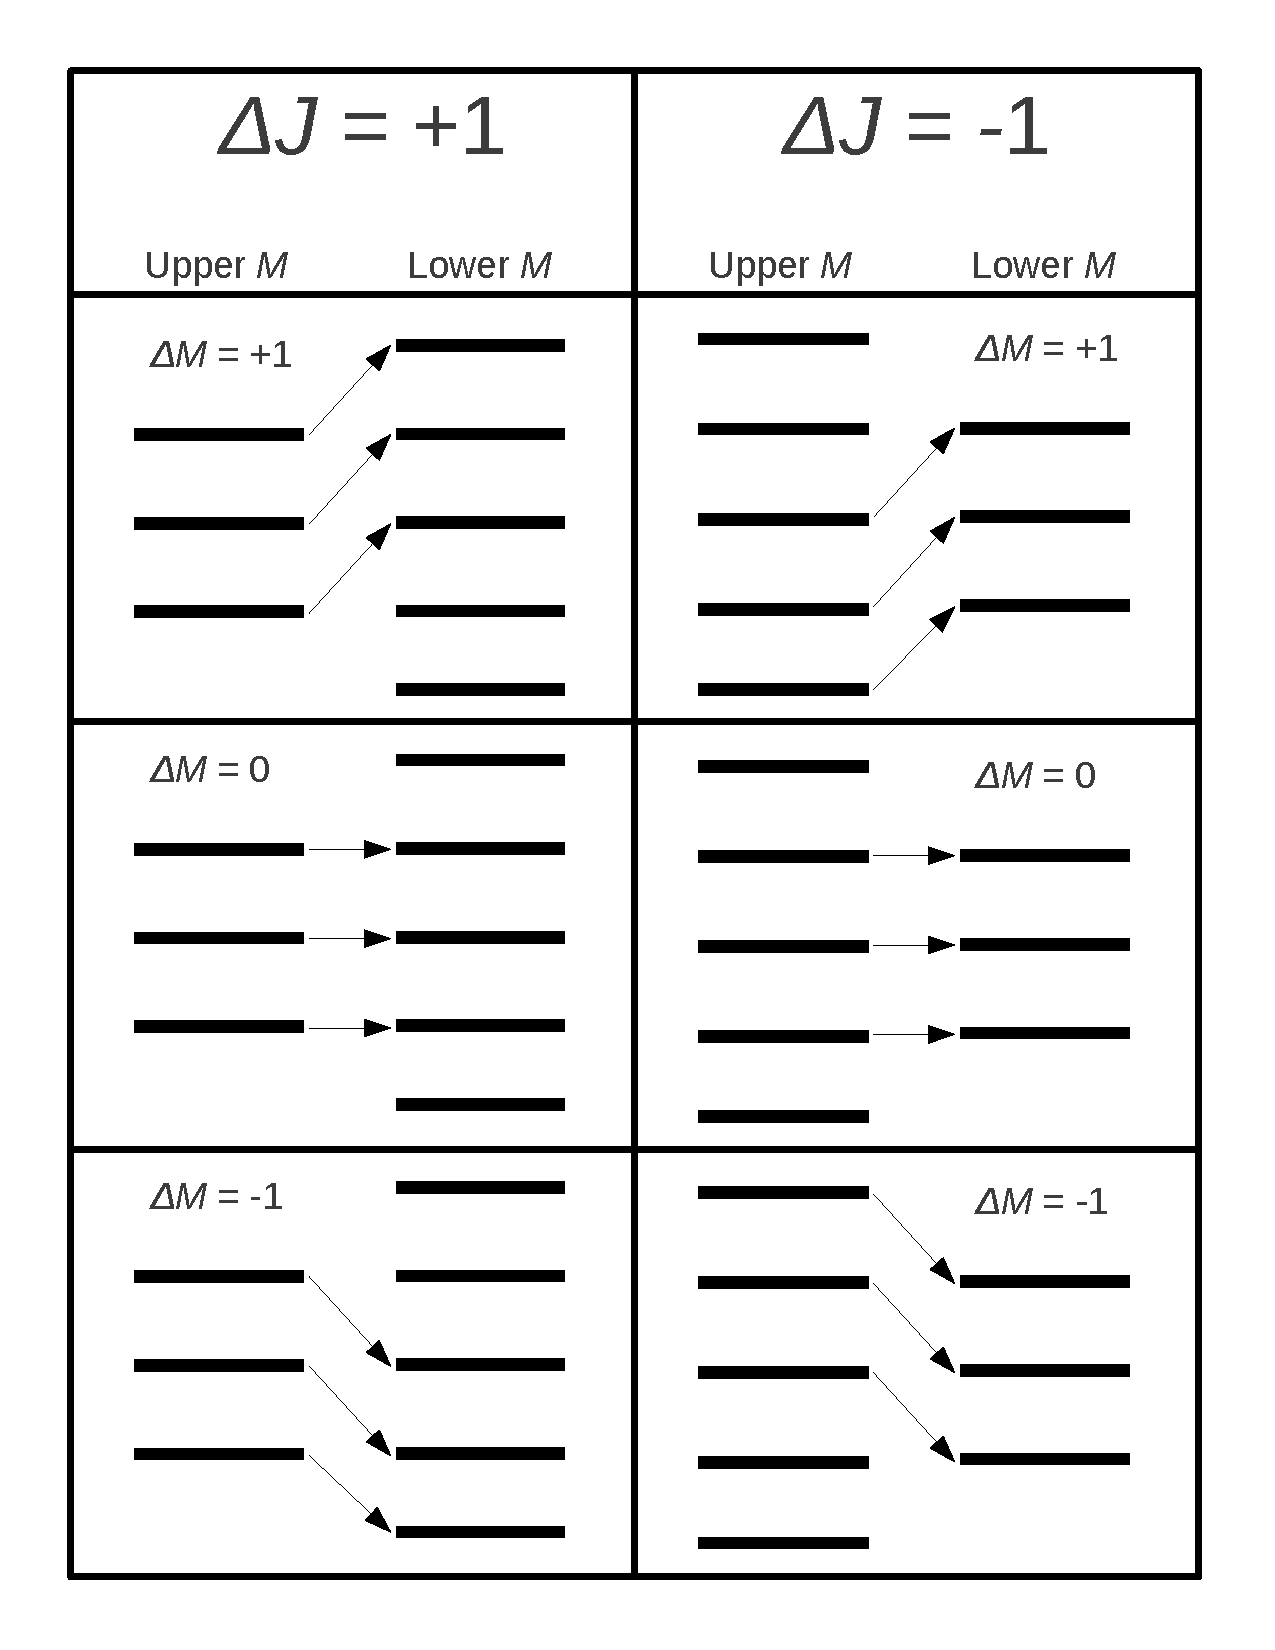
\includegraphics[width=343pt,keepaspectratio=true]{Selection_Rule.pdf}
 \begin{minipage}{312pt}
\vspace*{-0.8cm}
 \caption{Graphical representation of the selection rule. Note how the initial magnitude (denoted "Upper") of $M$ may be larger for the $N^{-}$ or $\Delta J = -1$ case. The initial value of $M$ is used in Tables~\ref{tab:delta_nu_0}~and~\ref{tab:zeta}, and consequently in Equation~\ref{eq:abs_zeeman_mat}.}
 \label{fig:zeeman_schematic}
\end{minipage}
\end{figure}

From Halliday, 1955, there are mainly two quantum numbers which govern the magnetism of particles. 
The first is the total orbital angular moment number for all electrons $N$. The second is the total spin angular moment number for all the electrons $S$. 
These two can be described by the spin-orbit coupling number $J$, which may be thought of as the total angular moment number of the particle. The oxygen molecule have $S=1$ due to the free electron pair, which means
the spin-orbit coupling number may take on two values for every $N$ such that $J=N\pm1$. 
In a magnetic field, the projection of $J$ on this field may take on a finite number of projected angular moment numbers $M = -J,\;1-J,\;(\cdots),\;J-1,\;J$. 
The projected angular moment influence the energy of the level by a factor $g_JMH$, where $H$ is the magnitude of the magnetic field and $g_J$ is known as the Landé splitting factor.

It is important to note that it only makes sense to classify the problem in the manner above if there is a coupling between $N$ and $S$. For sufficiently large magnetic fields, $N$ and $S$ uncouples and the problem complicates further. If even nuclear spin is considered and hyperfine transitions are allowed, yet another level is added to the problem (see, e.g., Halliday, 1955).

According to Lenoir, 1968, the rules of transition from initial to final state for oxygen only allow $\Delta J =\pm 1$ and $\Delta M = 0, \pm 1$. A transition with $\Delta J = +1$ is called an $N^+$ transition and a transition with $\Delta J = -1$ is called an $N^-$ transition. A simple schematic of the allowed transitions can be found in Figure~\ref{fig:zeeman_schematic}. There is a relative strength to each of the possible transitions displayed by the variable $\zeta$ (values in Table~\ref{tab:zeta}), and a shift in frequency, $\Delta\nu_0$, displayed by Table~\ref{tab:delta_nu_0}. It seems common for absorption databases (e.g., HITRAN) to list the central line frequency for every $J$ and let the user calculate the shifted frequency due to the magnetic field and $M$. Rewriting Equation~\ref{eq:abs_coeff} to take into account the Zeeman effect for oxygen gives
\begin{equation}\label{eq:abs_zeeman_mat}\scriptsize
 \mbox{\boldmath${\alpha}$}(\nu)=\frac{1}{2}nS(T)\!\!\!\sum_{M,\Delta M} \Bigl\{ \, \zeta(N,M,\Delta J, \Delta M) \; F(\nu, \nu_0 + \Delta\nu_0[N,M,\Delta J, \Delta M, H]) \; \mbox{\boldmath${K}'$}(\theta, \eta,\Delta M) \, \Bigr\}.
\end{equation}
Term by term we know what $n$, $S(T)$, $F(\nu,\nu_0)$, $\zeta$ and $\Delta\nu_0$ are supposed to represent. The magnitude of the magnetic field is denoted $H$. The factor $\frac{1}{2}$ is due to normalization issues and could be incorporated into $\zeta$ if need be. It is however kept in the theory for consistency with the tabular values of Liebe and Hufford (1989). 

The additional term, {\boldmath$K'$}, is due to the polarization that occurs in a plane made from the direction of propagation of the radiation, {\boldmath$n$}, due to the Zeeman effect. The angles involved are $\theta$ between the magnetic field {\boldmath$H$} and {\boldmath$n$}, and $\eta$ between $\mbox{\boldmath$H$}-\mbox{proj}_{\mbox{\boldmath$n$}}\left(\mbox{\boldmath$H$}\right)$ and the horizontal polarization direction used by ARTS {\boldmath$e$}$_h$. Both {\boldmath$n$} and {\boldmath$e$}$_h$ are defined and explained in Chapter~\ref{sec:polarization}.

Non-Zeeman affected species simply have an absorption matrix {\boldmath$\alpha$\unboldmath$=\alpha$\boldmath$I$\unboldmath}, where {\boldmath$I$} is the identity matrix of appropriate size.

\begin{table}[ht!]
 \centering
\begin{minipage}{280pt}
  \begin{tabular}{l|ll}
    \hline\\[-5pt]
    &$N^+$ transition&$N^-$ transition\\[5pt]\hline\\[-5pt]
    $\Delta M = +1$&$\frac{KH}{N+1}\left(1 +M\frac{N-1}{N}\right)$&$-\frac{KH}{N}\left(1 +M\frac{N+2}{N+1}\right)$\\[10pt]
    $\Delta M =  0$&$\frac{KH}{N+1}M\frac{N-1}{N}$&$-\frac{KH}{N}M\frac{N+2}{N+1}$\\[10pt]
    $\Delta M = -1$&$\frac{KH}{N+1}\left(-1 +M\frac{N-1}{N}\right)$&$-\frac{KH}{N}\left(-1 +M\frac{N+2}{N+1}\right)$
    \\[5pt]\hline
  \end{tabular}
\caption{Frequency shift, $\Delta\nu_0$, due to the Zeeman effect. $H$ is the magnitude of the external field in Tesla and $K$ is a constant of $2.8026\times10^{10}$
for shifts in Hz. The quantum numbers are the initial state values. This table can be found in Lenoir~(1968).}
\label{tab:delta_nu_0}
\end{minipage}
\end{table}

Lenoir (1968) describes the rotating polarization matrices, {\boldmath$\rho$}, in coherency terms as
\begin{equation}
 \mbox{\boldmath$\rho$\unboldmath}_{\sigma\pm} = \left[
\begin{array}{cc}
 1&\mp i\cos\theta\\
\pm i\cos\theta&\cos^2\theta
\end{array}
\right]\label{eq:rho_sigma}
\end{equation}
and
\begin{equation}
 \mbox{\boldmath$\rho$\unboldmath}_{\pi} = \left[
\begin{array}{cc}
 0&0\\
0&\sin^2\theta
\end{array}
\right].\label{eq:rho_pi}
\end{equation}
The angle, $\theta$, is between the propagation direction of the radiation and the magnetic field vector. The relevant {\boldmath$\rho$}-matrix  depends on the $\Delta M$ transition type. If $\Delta M = \pm 1$ use {\boldmath$\rho$}$_{\sigma\pm}$ and if $\Delta M = 0$ use {\boldmath$\rho$}$_{\pi}$.

\begin{table}[ht!]
 \centering
\begin{minipage}{254.1pt}
  \begin{tabular}{l|cc}
    \hline\\[-5pt]
    &$N^{+}$ transition&$N^{-}$ transition\\[5pt]\hline\\[-5pt]
    $\Delta M = +1$	&$\frac{3(N+M+1)( N+M+2 )}{4( N+1 )( 2N+1 )( 2N+3 ) }$
		        &$\frac{3( N-M-1 ) ( N-M ) }{ 4 N ( 2N+1 )( 2N-1 ) }$\\[10pt]
    $\Delta M =  0$	&$\frac{3  \left[(N+1)^2  - M^2 \right]}{ ( N+1 )  ( 2N+1 )  ( 2N+3 ) }$
			&$\frac{3 ( N^2 - M^2 )}{ N  ( 2N+1 )  ( 2N-1 ) }$\\[10pt]
    $\Delta M = -1$	&$\frac{3 ( N-M+1 )  ( N-M+2 ) }{ 4 ( N+1 )  ( 2N+1 )  ( 2N+3 )}$
			&$\frac{3 ( N+M-1 ) ( N+M )}{ 4 N  ( 2N+1 )  ( 2N-1 ) }$
    \\[5pt]\hline
  \end{tabular}
\caption{Strength of the individual, shifted, lines as determined by $\zeta$.
The quantum numbers are the initial state values. This table is adapted from Liebe and Hufford (1989).}
\label{tab:zeta}
\end{minipage}
\end{table}

To get the polarization matrix for a Stokes vector requires a bit of rewriting. First of all the coherency matrix for average signals following von Engeln (2000) is
\begin{equation}
 \mathbf{S} = \frac{1}{2}\sqrt{\frac{\epsilon}{\mu}} \left[
\begin{array}{cc}
 <E_v E_v^\ast>&<E_v E_h^\ast>\\
 <E_h E_v^\ast>&<E_h E_h^\ast>
\end{array}
\right].
\end{equation}

Looking at Equations~\ref{eq:polarization:stokesparam_I_general}~to~\ref{eq:polarization:stokesparam_V_general} we see that there should be a transformation possible such that the coherency matrix is described in Stokes parameters. This transformation
\begin{equation}\label{eq:coh_to_zee}\tiny
\frac{1}{2}\sqrt{\frac{\epsilon}{\mu}}
  \left[
    \begin{array}{cc}
      <E_v E_v^\ast>&<E_v E_h^\ast>\\
      <E_h E_v^\ast>&<E_h E_h^\ast>
    \end{array}
  \right] 
\Rightarrow
\frac{1}{2}\sqrt{\frac{\epsilon}{\mu}}
  \left[
    \begin{array}{cccc}
      &&<E_v E_v^\ast>+<E_h E_h^\ast>\\
      &&<E_v E_v^\ast>-<E_h E_h^\ast>\\
      -&(&<E_v E_h^\ast>+<E_h E_v^\ast>&)\\
      i&\left(\right.&<E_h E_v^\ast>-<E_v E_h^\ast>&\left.\right)
    \end{array} 
  \right].
\end{equation}
should hold for all radiation matrices \boldmath$S$\unboldmath. In other words, if we apply the radiative transfer
equation for the coherency case it will transform into Stokes parameters by Equation~\ref{eq:coh_to_zee}. The radiative transfer equation from Lenoir (1968) combined with the equation used herein (for pure absorption) gives 
$$\mbox{\boldmath$GS +SG^{t^\ast}$\unboldmath$ \Rightarrow $\boldmath$K$}I,$$
where {\boldmath$G$} is one of Equations~\ref{eq:rho_sigma}~or~\ref{eq:rho_pi} depending on $\Delta M$. This means that {\boldmath$G^{t^\ast} = G$}, which significantly simplifies the calculations to come.

One way to write the coherency matrix in Stokes parameters, $I_n$, is
\begin{equation}
 \mbox{\boldmath$S$} = \frac{1}{2}\sum_{n=0}^{n=3}\mbox{\boldmath$a$}_nI_n,\label{eq:a_iI_i}
\end{equation}
where it can be seen, e.g. from the transformation Equation~\ref{eq:coh_to_zee}, that
\begin{equation}\small
 \mbox{\boldmath$a$}_0 = \left[\begin{array}{cc}
       1&0\\0&1 
       \end{array}\right], \mbox{ }
 \mbox{\boldmath$a$}_1 = \left[\begin{array}{cc}
       1&0\\0&-1 
       \end{array}\right], \mbox{ }
 \mbox{\boldmath$a$}_2 = \left[\begin{array}{cc}
       0&-1\\-1&0 
       \end{array}\right]\mbox{ and }
 \mbox{\boldmath$a$}_3 = \left[\begin{array}{cc}
       0&i\\-i&0 
       \end{array}\right].
\end{equation}

Now applying the radiative transfer equation on the simplified radiation coherency matrix 
\begin{equation}\footnotesize
\mbox{\boldmath$S$}' = \frac{1}{2}(\mbox{\boldmath$G$}\mbox{\boldmath$a$}_0+\mbox{\boldmath$a$}_0\mbox{\boldmath$G$})I_0 + \frac{1}{2}(\mbox{\boldmath$G$}\mbox{\boldmath$a$}_1+\mbox{\boldmath$a$}_1\mbox{\boldmath$G$})I_1 + \frac{1}{2}(\mbox{\boldmath$G$}\mbox{\boldmath$a$}_2+\mbox{\boldmath$a$}_2\mbox{\boldmath$G$})I_2 + \frac{1}{2}(\mbox{\boldmath$G$}\mbox{\boldmath$a$}_3+\mbox{\boldmath$a$}_3\mbox{\boldmath$G$})I_3,
\end{equation}
gives us a straightforward way of deriving {\boldmath$K$}, since we now can treat each Stokes parameter separately as

$I_0'$:
\begin{equation}\label{eq:zeeman_stokes0}
 \left[
\begin{array}{cc}
G_{11}	&	G_{12}\\
G_{21}	&	G_{22}
\end{array}
\right] \times I_0
 \Rightarrow
\left[
\begin{array}{c}
G_{11}+G_{22}\\
G_{11}-G_{22}\\
-(G_{21}+G_{12})\\
i(G_{21}-G_{12})
\end{array}
\right] \times I_0
\end{equation}

$I_1'$:
\begin{equation}\label{eq:zeeman_stokes1}
 \left[
\begin{array}{cc}
G_{11}	&	0\\
0	&	-G_{22}
\end{array}
\right] \times I_1
 \Rightarrow
\left[
\begin{array}{c}
G_{11}-G_{22}\\
G_{11}+G_{22}\\
0\\
0
\end{array}
\right] \times I_1
\end{equation}

$I_2'$:
\begin{equation}\label{eq:zeeman_stokes2}
 -\frac{1}{2}\left[
\begin{array}{cc}
G_{21}+G_{12}	&	G_{11}+G_{22}\\
G_{11}+G_{22}	&	G_{21}+G_{12}
\end{array}
\right] \times I_2
 \Rightarrow
\left[
\begin{array}{c}
-(G_{21}+G_{12})\\
0\\
G_{11}+G_{22}\\
0
\end{array}
\right] \times I_2
\end{equation}

$I_3'$:
\begin{equation}\label{eq:zeeman_stokes3}
 \frac{1}{2}\left[
\begin{array}{cc}
 iG_{21}-iG_{12}	&	iG_{11}+iG_{22}\\
-iG_{11}-iG_{22}	&	iG_{21}-iG_{12}
\end{array}
\right] \times I_3
 \Rightarrow
\left[
\begin{array}{c}
i(G_{21}-G_{12})\\
0\\
0\\
G_{11}+G_{22}
\end{array}
\right] \times I_3
\end{equation}

Combining Vectors~\ref{eq:zeeman_stokes0}~to~\ref{eq:zeeman_stokes3} as column vectors will give the polarization rotation matrix
\begin{equation}
 \mbox{\boldmath$K$} = \left[
\begin{array}{cccc}
G_{11}+G_{22}&G_{11}-G_{22}&-(G_{21}+G_{12})&i\left(G_{21}-G_{12}\right)\\
G_{11}-G_{22}&G_{11}+G_{22}&0&0\\
-(G_{21}+G_{12})&0&G_{11}+G_{22}&0\\
i\left(G_{21}-G_{12}\right)&0&0&G_{11}+G_{22}
\end{array}
\right].
\end{equation}
This is favorably rewritten in terms of $\sigma_\pm$ and $\pi$ transitions such that
\begin{equation}
 \mbox{\boldmath$K$}_{\sigma\pm} = \left[
\begin{array}{rrrr}
1+\cos^2\theta&\sin^2\theta&0&\mp2\cos\theta\\
\sin^2\theta&1+\cos^2\theta&0&0\\
0&0&1+\cos^2\theta&0\\
\mp2\cos\theta&0&0&1+\cos^2\theta
\end{array}
\right]
\end{equation}
and
\begin{equation}
 \mbox{\boldmath$K$}_{\pi} =
\left[
\begin{array}{rrrr}
\sin^2\theta&-\sin^2\theta&0&0\\
-\sin^2\theta&\sin^2\theta&0&0\\
0&0&\sin^2\theta&0\\
0&0&0&\sin^2\theta
\end{array}
\right].
\end{equation}

These {\boldmath$K$}-matrices are however in a magnetic field dependent coordinate system. Since ARTS is using the coordinate system by Mishchenko et al. (2002), we simply rotate the coordinate system by so that the horizontal direction is
$$\mbox{\boldmath$R$}_{11} = \mbox{\boldmath$H$}-\mbox{\textbf{proj}}\mbox{\boldmath$_n$}\mbox{\boldmath$H$}$$
then the angle, $\eta$, between $\mbox{\boldmath$R$}_{11}$ and $\mbox{\boldmath$e$}_{h}$ can be used together with the coordinate system rotation matrix
\begin{equation}
 \mbox{\boldmath$L$}(\eta) = 
\left[
\begin{array}{rrrr}
 1&0&0&0\\
0&\cos 2\eta& -\sin 2\eta&0\\
0&\sin 2\eta& \cos 2\eta &0\\
0&0&0&1
\end{array}
\right]
\end{equation}
to determine that the polarization rotation matrices are
\begin{equation}\small
 \mbox{\boldmath$K$}'_{\pm\sigma}(\theta,\eta) = \left[
\begin{array}{rrrr}
1+\cos^2\theta & \cos\left(2\eta\right)\sin^2\theta &  \sin\left(2\eta\right)\sin^2\theta&\mp 2\cos\theta\\
\cos\left(2\eta\right)\sin^2\theta&1+\cos^2\theta&0&0\\
\sin\left(2\eta\right)\sin^2\theta&0&1+\cos^2\theta&0\\
\mp 2\cos\theta&0&0&1+\cos^2\theta
\end{array}
\right]
\end{equation}
and
\begin{equation}\small
 \mbox{\boldmath$K$}'_\pi(\theta,\eta) = \left[
\begin{array}{rrrr}
\sin^2\theta & -\cos\left(2\eta\right)\sin^2\theta &  -\sin\left(2\eta\right)\sin^2\theta&0\\
-\cos\left(2\eta\right)\sin^2\theta&\sin^2\theta&0&0\\
-\sin\left(2\eta\right)\sin^2\theta&0&\sin^2\theta&0\\
0&0&0&\sin^2\theta
\end{array}
\right].
\end{equation}

We have in this subsection derived the formalism for the Zeeman effect and may now use Equation~\ref{eq:abs_zeeman_mat} instead of Equation~\ref{eq:abs_coeff} to describe absorption when appropriate.

\subsection{Line-specific data and line catalogue data in ARTS} 

ARTS has an internal representation of spectral line data that maps
naturally to a native catalogue format, which we will discuss
below. This internal catalogue data exists and can be
handled in two variants, the so-called ARTSCAT-3 and ARTSCAT-4 -- versions~3
and 4 of the ARTS catalogue format. The spectroscopic databases commonly
used in Earth atmospheric research contain the spectroscopic parameters
representative for Earth conditions. This regards particular the foreign
broadened width, often called the air broadened width as it considerers
the contribution from nitrogen and oxygen that make up for the vast majority
of gases in the Earth atmosphere, and the pressure shift. ARTSCAT-3 contains
these ``classical'' spectroscopic parameters. ARTSCAT-4 on the other hand has
been developed with view on planetary science. That is, it holds these
parameters separately for the different molecular species. Theoretically this
has to list all cross-combinations of species. However, most species show only
very low abundances and can safely be neglected. For now, the main atmospheric
constituents of Earth, Mars, Venus, and Jupiter, namely N2, O2, H2O, CO2, H2,
and He are considered in the database.
It should be noted, that both line data formats can behandled simultaneously
within one calculation (writing to file of mixed format data, however, is not
possible).

Besides its own internal format, ARTS can also read several other catalogue
formats, in particular HITRAN and JPL format. If these other catalogues are used,
line data are converted to the internal ARTSCAT-3 representation during
reading. In other words, all unit conversions are done by the reading
routines.

The ARTS internal spectral line data files (both ARTSCAT-3 and -4) contain
an XML header and footer, and between them one entry for each spectral line.
Each entry starts with with an `@' character. It then contains the different line
parameters, separated by one or more blank characters. Scientific
notation is allowed, e.g. 501.12345e9.  

In contrast to other catalogues that are optimized for processing with
programs written in the FORTRAN language, ARTS does not use fixed
column widths. The advantage of this is that the precision of the
parameters is not limited by the format.

The first column of each entry contains the species and isotopologue,
following the naming scheme described below. Note that the intensity
is per molecule, i.e., it does not contain the isotopologue ratio. This is
similar to JPL, but different to HITRAN.
The definition of the further entries differ between the two ARTSCAT
representations.

\paragraph*{ARTSCAT-3 line format is:}
\begin{code}

Col  Variable                     Label    Unit     
-----------------------------------------------      
 0   `@'                         ENTRY        -     
 1   molecule & isotopologue tag  NAME        -
 2   center frequency                F       Hz     
 3   pressure shift of F           PSF    Hz/Pa    
 4   line intensity per molecule    I0   m^2/Hz     
 5   reference temp. for I0       T_I0        K
 6   lower state energy           ELOW        J    
 7   air broadened width          AGAM    Hz/Pa     
 8   self broadened width         SGAM    Hz/Pa
 9   AGAM temp. exponent          NAIR        -     
10   SGAM temp. exponent         NSELF        - 
11   ref. temp. for AGAM, SGAM   T_GAM        K
12   number of aux. parameters   N_AUX        -
13   auxiliary parameter          AUX1        -
14   ... 
15   error for F                    DF       Hz
16   error for I0                  DI0        %
17   error for AGAM              DAGAM        %
18   error for SGAM              DSGAM        %
19   error for NAIR              DNAIR        %
20   error for NSELF            DNSELF        %
21   error for PSF                DPSF        %

\end{code}
The parameters 0-12 must be present, the others can be missing, since
they are not needed for the calculation. For the error fields (15-21),
a $-1$ means that no value exists.

Some species may need special parameters that are not needed by other
species (for example overlap coefficients for $O_2$). In the case of
oxygen two parameters are sufficient to describe the overlap, but
other species, e.g., methane, may need more coefficients. The default
for \texttt{N\_AUX} is zero. In that case, no further \texttt{AUX}
fields are present.

\paragraph*{The line format of ARTSCAT-4 is:}
\begin{code}

Col  Variable                        Label    Unit
--------------------------------------------------
 0   `@'                             ENTRY       -
 1   molecule & isotopologue tag      NAME       -
 2   center frequency                    F      Hz
 3   line intensity                     I0  Hz*m^2
 4   reference temp. for I0           T_I0       K
 5   lower state energy               ELOW       J
 6   Einstein A-coefficient              A     1/s 
 7   Upper state stat. weight      G_upper       -
 8   Lower state stat. weight      G_lower       -
 9   broadening parameter self  GAMMA_self   Hz/Pa
10   broadening parameter N2      GAMMA_N2   Hz/Pa
11   broadening parameter O2      GAMMA_O2   Hz/Pa
12   broadening parameter H2O    GAMMA_H2O   Hz/Pa
13   broadening parameter CO2    GAMMA_CO2   Hz/Pa
14   broadening parameter H2      GAMMA_H2   Hz/Pa
15   broadening parameter He      GAMMA_He   Hz/Pa
16   GAM temp. exponent self        N_self       -
17   GAM temp. exponent N2            N_N2       -
18   GAM temp. exponent O2            N_O2       -
19   GAM temp. exponent H2O          N_H2O       -
20   GAM temp. exponent CO2          N_CO2       -
21   GAM temp. exponent H2            N_H2       -
22   GAM temp. exponent He            N_He       -
23   F pressure shift N2          DELTA_N2   Hz/Pa
24   F pressure shift O2          DELTA_O2   Hz/Pa   
25   F pressure shift H2O        DELTA_H2O   Hz/Pa   
26   F pressure shift CO2        DELTA_CO2   Hz/Pa   
27   F pressure shift H2          DELTA_H2   Hz/Pa   
28   F pressure shift He          DELTA_He   Hz/Pa   
29   Vib. & rotational assignments     VRA       -                      

\end{code}
Parameters 0-28 must be present. Parameter 29 contains coded quantum numbers.
The coding conventions are species specific. The definitions are given in file
\shortcode{ARTSCAT-4\_Col29\_Conventions.txt}, which is available along with
the first incarnation of an ARTSCAT-4 type spectroscopic catalog from the
\shortcode{arts-xml-data} data package.


\subsection{Species-specific data in ARTS}

A line absorption species in ARTS is a particular isotopologue of a
particular molecule.  Quantities such as the molecular mass and the
isotopologue ratio are specific and constant for each species.  Here is a
list of all species-specific information that is needed:
\begin{itemize}
\item Molecule name
\item Isotopologue name
\item Isotopologue ratio
\item Molecular mass
\item Corresponding tag in different catalogues (MYTRAN, HITRAN, JPL)
\item Partition function data
\end{itemize}

These data are currently stored in two source code files,
\fileindex{species\_data.cc} and \fileindex{partition\_function\_data.cc}. 
That is, currently these data are hard-coded and can not be changed via
controlfile settings.
In order to allow calculations for other planets, we are going to change
this in the not too far future, at least for the isotopologue ratios. It is
planned, that the data will then be read from include files instead.

\citet{buehler:artst:05} contains an explicit list of species that
were implemented at the time of writing of that article.  We do not include
such a list here, because it is hard to maintain. Instead, we directly refer
the user to check for the implemented species directly in file
\shortcode{species\_data.cc}. There, also the different sources of data
are documented.

\subsubsection{Partition function data}

ARTS uses third order polynomials to approximate partition functions,
so four polynomial coefficients have to be stored for each isotopologue
species. These data is stored in file
\fileindex{partition\_function\_data.cc}. The file also contains
documentation, including the source of the data for the different species.

The consistency of partition function data from different sources, and
the impact of partition function errors on sub-millimeter wave limb
sounder retrievals, was studied in detail in \citet{cverdes:05}. The
partition function data collection in ARTS is based on that study.

In general, the data in general are derived from the following sources:
\begin{description}
\item[TIPS:] Default.
\item[JPL:] Only species (including individual isotopologues) not covered by TIPS.
\item[Agnes Perrin:] Personal communication, only for species BrO.
\end{description}

The TIPS program is developed and maintained by B. Gamache. In conjunction
with HITRAN it is the suggested way to derive the partition functions and is part of the HITRAN distributions. More recent versions might be available via B. Gmache's website (\url{http://faculty.uml.edu/robert_gamache/}, `Software and Data' section). TIPS covers all molecular species and isotopolgues found in the respective version of the HITRAN database. Often it includes some more species than HITRAN, and extensions for other species (e.g., species of astrophysical interest) can be derived from the Gamache website.

Earlier versions of TIPS (until at least 1997) provided 3rd order polynomial
coefficients, which were then used in ARTS.
Newer versions (from at latest 2003) provide partition
functions for a specific molecule and isotopologue at a specific temperature,
and tabulated values can be obtained through successive runs of the program.
Polynomial coefficients then need to be derived by a fit to the TIPS output.
Here, partition functions were calculated on a 1K-step grid, and the polynomial
coefficients derived by a least-square fit between 150\,--\,300\,K (unless
otherwise noted in \fileindex{partition\_function\_data.cc}).

The coefficients for the few species which are not covered in
TIPS are calculated from JPL values. The JPL catalogue has a
different way to calculate the partition function. It provides the
partition function at a set of specific temperatures: 300, 225, 150, 75, 37.5,
18.75, 9.375 K. An interpolation scheme is given for values
inbetween: the partition functions are assumed to be proportional to $T^{1.5}$
for non-linear molecules (degrees of freedom: 3) and proportional to $T$ for
linear molecules (degrees of freedom 2).
From these data polynomial coefficients are derived in the same way as from TIPS
output: first, partition functions are tabulated on a 1K-step grid, then a
least-square fit over T\,=\,150\,--\,300\,K is performed.

The partition function data for BrO were provided by Agnes
Perrin, Orsay, France.

The temperature range used for deriving the polynomial fit was judged to be
representative of the range of temperatures occuring in the Earth atmosphere.
For calculations in planetary atmospheres it might be advantageous being able to
use other data, e.g. such derived for temperatures prevailing there. We are
exploring options to allow for that (e.g., read data from include files as
planned for isotopologue ratios, or replacement of parameterized partition
functions by directly calculated one through embedding TIPS and the JPL scheme
in ARTS).

% ================================================================================
% The following section was originally written by Thomas Kuhn, iup Bremen, tkuhn@uni-bremen.de
% ================================================================================

\section{Continuum absorption}
\label{sec:abs_theory:ContAbs}
% ===========================

As pointed out above, some molecules show beside the resonant line
absorption also non-resonant continuum absorption. The main qualitative
difference is the smooth dependence on frequency of the non-resonant
absorption part in contrast to the resonant absorption part who shows 
strong local maxima and minima.

The implemented continuum absorption modules are connected with water
vapor ($\hzo$), oxygen ($\oz$), nitrogen ($\nz$), and carbon dioxide
($\coz$). Since these molecules have various permanent electric or magnetic
multipoles, the physical explanations for the continuum absorption is 
different for each of these molecules.

Water Vapor has a strong electric dipole moment and posses therefore a 
wealth of rotational transitions in the microwave up to the submillimeter 
range. One explanation for the $\hzo$-continuum absorption is the inadequate 
formulation of the far wings of a spectral line, since the usually employed 
\citet{vanvleck:45} line shape is according to its derivation only valid 
in the near wing zone. Other explanations are (see \citet{pwr:93} for details) 
far wing contribution from far-infrared water vapor lines, collision induced 
absorption (CIA), and water polymer absorption. At present one can not definitively 
decide which of these possibilities is the correct one, probably all of them 
play a more or less important role, depending on the frequency range.

Oxygen is special, because it has no permanent electric dipole moment,
but a permanent magnetic dipole moment. The aligned spins of the two
valence electrons gives a $^{3}\Sigma$ ground state of molecular
oxygen.  Due to the selection rules for magnetic dipole transitions,
transitions with resonance frequency equal to zero are allowed. Such
transitions have a characteristic Debye line shape function.

The homonuclear nitrogen molecule has in lowest order an electric quadrupole moment 
of modest magnitude.
For the frequency range below 1\,THz the collision induced rotation absorption 
band \citep{goodyandyung:89} is of most importance. The band center is around 3\,THz and 
at 1\,THz the band strength is approximately 1/6 of the maximum value (see 
Figure 5.2 of \citet{goodyandyung:89}). The electric field of the quadrupole 
moment of one molecule induces a dipole moment in the second molecule. This allows 
rotational transitions according to the electric quadrupole selection rules, 
$|\Delta\,J|=$0,2 (see \citet{pwr:93} for details). 

In a similar way, carbon dioxide also exhibits a collision induced
absorption band (maximum around 1.5\,THz, Figure 5.10 of
\citet{goodyandyung:89}). Characteristic for collision induced
absorption is the dependency on the square of the molecular density.



\subsection{Water vapor continuum models}
\label{leveld:h2o_Cont}
%------------------------------------
As shown by \citet{liebeandlayton:87}, \citet{pwr:98}, and \citet{ma:90},
the water vapor continuum absorption can be well described by 
\begin{equation} 
  \label{eq:abs_theory:abs_cont}
  \alphac = \nu^2 \cdot \Theta^{3} \cdot 
            (\cso \cdot \phzo^2 \cdot \Theta^{\xs} + 
             \cdo \cdot \phzo \cdot \pda \cdot \Theta^{\xf})
\end{equation}
where the microwave approximation ($h\nu\ll k_BT$ ) of the radiation field term 
is already applied. The adjustment of Eq. \ref{eq:abs_theory:abs_cont} to the data 
is performed through the parameter set $\cso$, $\xs$, $\cdo$, and $\xf$. 
Table \ref{tab:wvcontparam} gives some commonly used continuum parameter sets.
\begin{table}[!hbt]
  \begin{center}
  \begin{tabular}{lrrrrr}
    \hline
    model  & \multicolumn{1}{c}{$\cso$} & 
             \multicolumn{1}{c}{$\xs$}  & 
             \multicolumn{1}{c}{$\cdo$} & 
             \multicolumn{1}{c}{$\xd$}  & 
             ref.\\
           & \multicolumn{1}{c}{$\left[\frac{\mbox{dB/km}}
                               {\mbox{hPa}^2~\mbox{GHz}^2}\right]$} & 
             \multicolumn{1}{c}{$[1]$} & 
             \multicolumn{1}{c}{$\left[\frac{\mbox{dB/km}}
                               {\mbox{hPa}^2~\mbox{GHz}^2}\right]$} & 
             \multicolumn{1}{c}{$[1]$} & \\
    \hline
%    MPM85  & 4.92$\cdot$10$^{-8}$ & 2.5 & 0.255$\cdot$10$^{-8}$  & -0.5 & \citet{liebe:85}\\
    MPM87  & 6.50$\cdot$10$^{-8}$ & 7.5 & 0.206$\cdot$10$^{-8}$  &  0.0 & \citet{liebeandlayton:87}\\
    MPM89  & 6.50$\cdot$10$^{-8}$ & 7.3 & 0.206$\cdot$10$^{-8}$  &  0.0 & \citet{liebe:89}\\
    CP98   & 8.04$\cdot$10$^{-8}$ & 7.5 & 0.254$\cdot$10$^{-8}$  &  0.0 & \citet{cruzpol:98}\\ 
    PWR98  & 7.80$\cdot$10$^{-8}$ & 4.5 & 0.236$\cdot$10$^{-8}$  &  0.0 & \citet{pwr:98}\\
    \hline
    MPM93$^*$ & 7.73$\cdot$10$^{-8}$ & 4.55 & 0.253$\cdot$10$^{-8}$  & 1.55 & \citet{liebeetal:93}\\
    \hline
 \end{tabular}
\end{center}
 \caption[Liebe-type continuum model parameters.]{Values of commonly used continuum parameter sets. The last line (MPM93$^*$)
   represents an approximation of the pseudo-line continuum of MPM93
   in the form of Eq. \ref{eq:abs_theory:abs_cont}.}
 \label{tab:wvcontparam}
\end{table}

\subsubsection{The MPM93 continuum parameterization}
\label{leveld:mpm93:contabs}
%-----------------------------------------------
In the MPM93 model \citep{liebeetal:93}, the water 
vapor continuum is treated as a pseudo-line located in the far infrared 
around 2\,THz. The pseudo-line continuum has therefore not four but seven 
parameters, the pseudo-line center frequency ($\nu^*$) and the six 
pseudo-line parameters ($\beks$,$\cdots$,$\bsks$):
%
\begin{eqnarray}
  \label{eq:abs_theory:mpm93:contabs}
  \alphampmnc & = & 0.1820 \cdot \frac{\beks}{\nu^*} \cdot \phzo \cdot 
                \Theta^{3.5} \cdot \exp{\left(\bzks\cdot(1-\Theta)\right)} \cdot 
                \nu^2 \cdot \shapec\\
%
  \label{eq:abs_theory:mpm93:contabs1}
   \shapec & = & \left[\frac{\gamc}{(\nu^*+\nu)^2+\gamc^2} + 
                       \frac{\gamc}{(\nu^*-\nu)^2+\gamc^2}\right]\\
%
  \label{eq:abs_theory:mpm93:contabs2}
  \gamc & = &  \bdks \cdot 
        \left(\bvks \cdot \phzo \cdot \Theta^{\bsks}~~+~~ 
                          \pda  \cdot \Theta^{\bfks}\right)\\
  \nonumber
\end{eqnarray}
%
Table \ref{tab:mpm93_cont_param} lists the values of this continuum 
parameter set. It is remarkable that all these parameters are much 
larger compared to the physical water vapor line parameters of the 
same model. The only exception is $\bzks$, the parameter 
which governs the exponential temperature behavior of the line strength. 
%
\begin{table}[!hbt]
  \begin{center}
  \begin{tabular}{rrrrrrr}
   \hline
   $\nu^*$ & $\beks$ & $\bzks$ & $\bdks$ & $\bvks$ & $\bfks$ & $\bsks$\\
   {\rm [GHz]}  & {[$\frac{\rm kHz}{\rm hPa}$]} & {\rm [1]} & 
   {[$\frac{\rm MHz}{\rm hPa}$]} & {\rm [1]} & {\rm [1]} & {\rm [1]} \\
    \hline
   1780.000 & 2230.000 & 0.952 & 17.620 & 30.50 & 2.00 & 5.00 \\
   \hline
  \end{tabular}
  \end{center}
  \caption{List of the MPM93 pseudo-line water vapor continuum parameters.}
  \label{tab:mpm93_cont_param}
\end{table}
%
The magnitude of the pseudo-line width is shown for four different 
cases in Table\,\ref{tab:mpm_psl_broad}. 
%
\begin{table}[!htb]
\begin{center}
\begin{tabular}{lrrr}
\hline
 & \multicolumn{2}{c}{contribution} & \multicolumn{1}{c}{total} \\
 & \multicolumn{1}{c}{$\hzo$--$\hzo$} & \multicolumn{1}{c}{$\hzo$--air} & \\
\hline
$\gamc$(200\,K) & 40.8\,GHz & 80.4\,GHz & 121.2\,GHz\\
$\gamc$(300\,K) &  5.4\,GHz & 23.0\,GHz &  28.4\,GHz\\
\hline
\end{tabular}
\caption[MPM93 parameters.]{Magnitude of the line width of the pseudo-line of the
  continuum term in MPM93. Assumed is a total pressure of 1000\,hPa
  and a water vapor partial pressure of 10\,hPa.}
\label{tab:mpm_psl_broad}
\end{center}
\end{table} 

This change of continuum parameterization makes it difficult 
to compare MPM93 with the models which use Eq. (\ref{eq:abs_theory:abs_cont}). 
However, with respect to microwave frequencies, the 
line shape function, $F_c(\nu)$, can be approximated since 
the magnitude of the pseudo-line width is much smaller compared to the 
distance between microwave frequencies and $\nu^*$, as 
shown for four different cases in Table\,\ref{tab:mpm_psl_broad}:
\begin{equation}
 \label{eq:abs_theory:mpm93:contfapp1}
 \shapec \approx 2 \cdot \frac{\gamc}{\nucc^2}
\end{equation}
Inserting Eq. (\ref{eq:abs_theory:mpm93:contfapp1}) into Eq. (\ref{eq:abs_theory:mpm93:contabs})
gives a quadratic frequency dependence of the MPM93 continuum,
similar to the continuum parameterization expressed in 
Eq. (\ref{eq:abs_theory:abs_cont}). By additionally approximating 
the temperature dependence to the simple form
\begin{eqnarray}
  \xs\cdot\ln{(\Theta)} & = & 
  \ln{\left(\Theta^{3.5} \cdot e^{\bzks\cdot(1-\Theta)}\right)}\nonumber\\
%
  \xs  & = & 3.5 +
  \bzks\cdot\frac{1-\Theta}{\ln{(\Theta)}}\nonumber\\
%
  \xs & \approx & 3.5 -\bzks = 2.55\hspace*{15mm}\mbox{with}\hspace*{2mm}
                 \ln{(\Theta)}\approx(\Theta-1)\\
\nonumber
\end{eqnarray}
%
one can rearrange the pseudo-line continuum to fit Eq. (\ref{eq:abs_theory:abs_cont})
(denoted by MPM93$^*$). The so deduced continuum parameter set is given in 
Table \ref{tab:wvcontparam}.\\
The MPM93$^*$ continuum parameters $\cso$ and $\cdo$ are 20\,\% and 
15\,\% larger, respectively, than in the case of MPM87/MPM89. 
Large discrepancies exist for the temperature exponents $\xs$ 
and $\xd$ between MPM93$^*$ and earlier model versions. The 
exponent $\xs$ is in MPM93$^*$ only 60\,\% of the corresponding 
value in MPM89 and the temperature dependence of the $\hzo$-air 
term is significant larger than for earlier MPM versions.
This reduction of $\xs$ is mainly due to additional measurements 
considered in MPM93 \citep{beckerautler:46,godonetal:92}, 
while the continuum parameters in MPM87/MPM89 are determined 
by a single laboratory measurement at 138\,GHz.



\subsection{Oxygen continuum absorption}
\label{levelc:o2cont}
%-----------------------------------
As pointed out by \citet{vv:87}, the standard theory for
non-resonant absorption is that of Debye (see also \citet{townes:55}). 
The Debye line shape is obtained from the VVW line shape function 
by the limiting case $\nuk \rightarrow 0$.
Both, \citet{liebeetal:93} and \citet{pwr:93} adopted the
Debye theory for their models. The only difference is the formulation
of the line broadening, where the influence of water vapor is treated 
slightly different: 
\begin{eqnarray}
  \label{eq:abs_theory:abs_cont_pwr_o2}
  \alphac &=&  C \cdot \pda \cdot \Theta^2 \cdot 
             \frac{\nu^2 \cdot \gamma}{\nu^2+\gamma^2}\\
  \label{eq:abs_theory:abs_cont_pwr_o2_1}
  \gamma &=&  w \cdot (\pda\cdot \Theta^{0.8} + 1.1 \cdot \phzo \cdot
  \Theta)\hspace*{5mm}:~\mbox{Rosenkranz}\\
  \label{eq:abs_theory:abs_cont_pwr_o2_2}
  \gamma &=&  w \cdot \ptot \cdot \Theta^{0.8}\hspace*{34mm}:~\mbox{MPM93}\\
\nonumber
\end{eqnarray}
where $\pda$ denotes the dry air partial pressure ($\pda=\ptot-\phzo$). 
The value for the strength is $C =$\,2.56$\cdot$10$^{-20}$\,1/(m\,Pa\,Hz) 
in the case of the Rosenkranz model and 
$C =$\,2.57$\cdot$10$^{-20}$\,1/(m\,Pa\,Hz) in the case of the MPM93 model.
The MPM93 value for $C$ is therefore about 0.4\,\% larger than in the 
Rosenkranz model. Since the volume mixing ratio of oxygen in dry air
is constant in the lower Earth atmosphere (0.20946 \citep{goody:95}), 
both models incorporate the oxygen $VMR$ ($\vmroz$) in the 
constant $C$. In the arts model the separation between the oxygen
$VMR$ and the constant $C$ is explicitely done. In this case follows:
\begin{eqnarray} 
 \label{eq:abs_theory:o2cont_const_vmr_1}
 C &=& 0.20946 \cdot \widehat{C}\\
 \label{eq:abs_theory:o2cont_const_vmr_2}
 \widehat{C} &=& 1.22\cdot 10^{-19}~\mbox{[1/(m\,Hz\,Pa)]\hspace{10mm}:~Rosenkranz} \\
 \label{eq:abs_theory:o2cont_const_vmr_3}
 \widehat{C} &=& 1.23\cdot 10^{-19}~\mbox{[1/(m\,Hz\,Pa)]\hspace{10mm}:~MPM93} 
\end{eqnarray} 
The width parameter $w$ is in both models the same, 
$w =$\,5.6$\cdot$10$^{3}$\,Hz/Pa. If we define the width $\gamma$ in a more 
general way like
\begin{equation} 
 \label{eq:abs_theory:o2_cont_gamma_general}
 \gamma = w \cdot \left( A \cdot \pda  \cdot \Theta^{n_d} + 
                   B \cdot \phzo \cdot \Theta^{n_w} \right) 
\end{equation}
we can fit both models, the Rosenkranz and the MPM93 model, into the 
same parameterization with ($A=1$, $B=1.1$, $n_d=0.8$, $n_w=1.0$) for 
the Rosenkranz model and ($A=1.0$, $B=1.0$, $n_d=0.8$, $n_w=0.8$) for 
MPM93.

The oxygen continuum absorption term is proportional to 
the collision frequency of a single oxygen molecule with other air molecules 
and thus proportional to the dry air pressure\footnote{The absorption
  due to weakly bound complexes of $\oz$--$X$ with $X=\hzo,~\nz$ is 
  treated separately and therefore not included in this Debye formula.}.




\subsection{Nitrogen continuum absorption}
\label{levelc:n2cont}
%-------------------------------------
Since molecular nitrogen has in its unperturbed state no electric or 
magnetic dipole moment (but an electric quadrupole moment), it shows 
no rotational spectral signature in the microwave region. Regardless 
of this, nitrogen absorbs radiation in this frequency range due to 
collision induced absorption (CIA). Far--infrared roto-translational
band structures from free--free interactions give rise to far wing
absorption below 1\,THz.

Different parameterizations of this absorption term for the 
frequency range below 1\,THz are available 
\citet{pwr:93,liebeetal:93,borysow:86}. Common to all these 
models is the quadratic dependency on $\nz$ partial pressure which is 
a direct consequence of the underlying CIA processes involved.
The simplest model is given by \citet{pwr:93}, which uses 
the same parameterization as for the water vapor continuum, described 
in Equation \ref{eq:abs_theory:abs_cont}:
\begin{equation}
  \label{eq:abs_theory:abs_cont_pwr_n2}
    \alphac =  C \cdot \nu^{n_{\nu}} \cdot \Theta^{n_T} \cdot \pnz^{n_p}
\end{equation}
with $C = 4.56\cdot 10^{-13}$ dB/(km\,hPa$^2$\,GHz$^2$), $n_{\nu}=$\,2, 
$n_T=$\,3.55, and $n_p=$\,2, respectively. The laboratory data set 
for the determination of $C$ is manly from \citet{dagg:75,dagg:78} 
around 70 and 140\,GHz, respectively.

The MPM models has compared with Equation \ref{eq:abs_theory:abs_cont_pwr_n2} 
an additional frequency dependent term which leads to the 
following expression
\begin{eqnarray}
  \label{eq:abs_theory:abs_cont_MPM89_n2}
    \alphac &=& \widehat{C} \cdot (1.0-1.2\cdot10^{-5}\cdot
               \nu^{1.5}) \cdot \nu^2 \cdot \Theta^{3.5} \cdot \pda^2
               \hspace*{10mm}:~\mbox{MPM89}\\
%
  \label{eq:abs_theory:abs_cont_MPM93_n2}
    \alphac &=& \widehat{C} \cdot \frac{\nu^2}{(1.0+a\cdot \nu^{n_{\nu}})} 
                \cdot \Theta^{3.5} \cdot \pda^2
                \hspace*{16mm}:~\mbox{MPM93}\\
          a &=&  
\nonumber
\end{eqnarray}
where the parameter is $\widehat{C} = 2.55\cdot 10^{-13}$ dB/(km\,hPa$^2$\,GHz$^2$), 
$a=$1.9$\cdot$10$^{-5}$\,GHz$^{-n_{\nu}}$, and $n_{\nu}=$\,1.5.
based on data from \citet{stankevich:74} and \citet{stonenw:84}. 
With respect to the 22\,GHz water vapor line, 
the additional frequency terms in brackets in 
Equations \ref{eq:abs_theory:abs_cont_MPM89_n2} and \ref{eq:abs_theory:abs_cont_MPM93_n2}
are nearly unity and therefore not essential. Therefore all
three parameterizations have the same frequency and temperature
relationship, but the absolute magnitude is in the case of Rosenkranz
80\,\% higher compared with the MPM models.

The model of Borysow and Frommhold\footnote{{the source code of this
    model can be downloaded from the home page of A. Borysow:}\\
  http://www.astro.ku.dk/$\sim$aborysow/} is somewhat different since
their focus is mainly on the radiative transfer in the Titan's
atmosphere with the infrared interferometer spectrometer, IRIS, on
board the Voyager Spacecraft. This detailed model is primarily
designed to parameterize each of the roto-translational spectral lines
around 200\,cm$^{-1}$ ($\approx$ 6\,THz) accurately. The analyzed data
set incorporate the data source used by the Rosenkranz but is largely
extended with measurements in the far--infrared.



\subsection{Carbon dioxide continuum absorption}
\label{levelc:co2cont}
%--------------------------------------------
\citet{pwr:93} gives a similar parameterization for the $\coz$-continuum 
absorption term as for the nitrogen continuum, with 
\begin{equation}
  \label{eq:abs_theory:abs_cont_pwr_co2}
    \alphac =   \cdot \nu^2 \cdot  
                \left[ C_s \cdot \pcoz^2           \cdot \Theta^{n_s} +
                       C_f \cdot \pcoz  \cdot \pnz \cdot \Theta^{n_f} \right]
\end{equation}
where the parameter values $C_s = 3.23\cdot 10^{-11}$
dB/(km\,hPa$^2$\,GHz$^2$), $C_f = 1.18\cdot 10^{-11}$
dB/(km\,hPa$^2$\,GHz$^2$), $n_s=5.08$, and $n_f=4.7$, respectively, 
are determined from laboratory measurements of \citet{ho:66,dagg:75}. 
Since the foreign term
includes only nitrogen as perturber, one can get an estimate for dry
air by replacing $\pnz$ by the dry air partial pressure in
Equation \ref{eq:abs_theory:abs_cont_pwr_co2}. Because nitrogen is usually a more
efficient perturber than oxygen, this estimation can be regarded as an
upper limit. Concerning the Earth's atmosphere, the foreign broadening
term is more interesting since the carbon dioxide partial pressure is
only approximately 0.04\,\% of the nitrogen partial pressure up to
90\,km.



% ================================================================================
% The following section was originally written by Thomas Kuhn, iup Bremen, tkuhn@uni-bremen.de
% ================================================================================



\section{Complete absorption models}
\label{sec:abs_theory:CompAbsMod}
% =================================
The MPM absorption model of Liebe and coworkers consists of modules for 
water vapor and oxygen absorption. The Rosenkranz (PWR98) absorption 
model include also $\hzo$ and $\oz$ while the Cruz-Pol et al. (CP98) absorption 
models include absorption due to water vapor. Additionally 
the CP98 model has a strongly reduced parameter set for the $\hzo$-line 
absorption since it is especially intended for the range around the 
22\,GHz water line. The MPM and R98 are valid from the microwave 
up to the submillimeter frequency range (1-1000\,GHz).

Implemented in ARTS are the following modules of the above mentioned models:
%
\begin{center}
\begin{tabular}{ll}
\hline
species & model\\
\hline
$\hzo$ & MPM87, MPM89, MPM93, PWR98, CP98 \\
$\oz$  & MPM93, PWR98 \\
\hline
\end{tabular}
\end{center}




\subsection{Complete water vapor models}
\label{levelc:CompWatVapMod}
% ==================================
In ARTS several complete water vapor absorption models are implemented and 
can easily be used. Implemented models are the versions 
MPM87 \citep{liebeandlayton:87}, MPM89 \citep{liebe:89}, and 
MPM93 \citep{liebeetal:93} of the Liebe Millimeter-wave Propagation Model 
and additionally the models of Cruz-Pol et al. (CP98) \citep{cruzpol:98} 
and P. W. Rosenkranz (PWR98) \citep{pwr:98}. 
MPM and PWR98 are especially desigend for fast absorption calculations in 
the frequency range of 1-1000\,GHz while the CP98 model is a reduced model 
for a narrow frequency band around the 22\,GHz $\hzo$-line (especially used 
by ground-based radiometers).

The total water vapor absorption ($\alphatot$) is in all the stated models 
described by a line absorption ($\alphal$) term and a continuum absorption 
($\alphac$) term: 
\begin{equation}
  \label{eq:abs_theory:h2o:totabs}
  \alphatot = \alphal + \alphac
\end{equation}
The main differences between the different models is the line shape used for 
$\alphal$ and the formulation of $\alphac$.

It has to be emphasized that, $\alphal$ and $\alphac$ of different
models are not necessarily compatible and should therefore not be 
interchanged between different models.


\subsubsection{MPM87 water vapor absorption model}
\label{leveld:mpm87}
%------------------------------------------
This version, which is described in \citet{liebeandlayton:87} and 
follows the general line of the MPM model to divide the total 
water vapor absorption, $\alphampmotot$, into a spectral line 
term, $\alphampmol$, and a continuum term not attributed to 
spectral lines, $\alphampmoc$:
\begin{equation}
  \label{eq:abs_theory:mpm87_abs}
  \alphampmotot = \alphampmol + \alphampmoc\hspace*{10mm}\mbox{dB/km}
\end{equation}



\paragraph{Water vapor line absorption:}
\label{levele:mpm87_h2olines}
%-----------------------------------
The MPM87 \citep{liebeandlayton:87} water vapor line catalog consists 
of 30 lines from 22\,GHz up to 988\,GHz. The center frequencies and parameter 
values are listed in Table \ref{tab:mpm87linelist}. To describe the line 
absorption, a set of three parameters ($\bek$ and $\bdk$) per line are used: two 
for the line strength and one for the line width. The total line 
absorption coefficient (in units of dB/km) is the sum over all 
individual line absorption coefficients\footnote{The factor 
  $0.1820 \cdot 10^{6}$ is equal to $(4\,\pi/c)\cdot 10\log{(e)}$
  (the term $(4\,\pi/c)$ comes from the definition of the absorption
  coefficient in terms of the dielectric constant and the term 
  $10\,\log{(e)}$ is due to the definition of the Decibel.) The
  velocity of light is defined as $c=2.9979\cdot 10^{-4}$\,km\,GHz. 
  The factor $10^{6}$ is incorporated into the line strength and 
  does therefore not appear in the pre-factor.}:
\begin{equation}
  \label{eq:abs_theory:mpm87:absline}
  \alphampmol = 0.1820 \cdot \nuk \cdot \phzo \cdot 
  \sum_{k}{\inten \cdot \shape}\hspace*{10mm}\mbox{dB/km}
\end{equation}
where $\inten$ is the line intensity described by the parameterization
\begin{equation}
  \label{eq:abs_theory:mpm87:strength}
  \inten = \bek \cdot \phzo \cdot \Theta^{3.5} 
           \cdot \exp{(\bzk \cdot [1-\Theta])}\hspace*{10mm}\mbox{kHz}
\end{equation}
with $\nuk$ as the line center frequency, $\phzo$ the water
vapor partial pressure and $\Theta = 300\,\mbox{K}/T$.\\
The line shape function, $\shape$, in Eq. (\ref{eq:abs_theory:mpm87:absline}) 
is the standard Van Vleck-Weisskopf (VVW) function, given by:
\begin{eqnarray}
% Van Vleck-Weisskopf function
  \label{eq:abs_theory:mpm87:VVW}
  \shape & = & \left(\frac{\nu}{\nuk}\right) \cdot 
               \left[\frac{\gamk}{(\nu - \nuk)^2 + \gamk^2} + 
                     \frac{\gamk}{(\nu + \nuk)^2 + \gamk^2}\right]\\
\end{eqnarray}
The pressure broadened line width, $\gamk$, is calculated with the 
single parameter $\bdk$ in the following way:
\begin{equation}
  \label{eq:abs_theory:mpm87:gamma}
  \gamk = \bdk \cdot 
          (4.80 \cdot \phzo \cdot \Theta^{1.1} + \pda \cdot
          \Theta^{0.6})\hspace*{10mm}\mbox{GHz}
\end{equation}
where $\pda$ is the partial pressure of dry air ($\pda=\ptot-\phzo$). 
The parameterizations of $\inten$ and $\gamk$ are already in use for the 
early version of MPM81 \citep{liebe:81}.
%
\begin{longtable}{rrrrr}
 K & K & K & K & K \kill
%
% --------------------- only begin of table ------------------------------
 \hline
       & $\nu_k$ & $\bek$   & $\bzk$ & $\bdk$  \\
% //      [GHz]    [kHz/kPa]   [1]     [GHz/kPa]
 $k$   & {\rm [GHz]}  & {[$\frac{\rm kHz}{\rm kPa}$]} & {\rm [1]} & 
 {[$\frac{\rm GHz}{\rm kPa}$]}\\
 \hline
 \endfirsthead
% --------------------- every page begin of table ------------------------
 \hline
  $k$  & $\nu_k$ & $\bek$ & $\bzk$ & $\bdk$ \\
 \hline
 \endhead
% --------------------- every page end of table ------------------------
 K & K & K & K & K \kill
 \hline
 \caption[]{(continued on next page)}\\
 \endfoot
% --------------------- only end of table ------------------------------
 K & K & K & K & K \kill 
 \hline
 \caption[MPM87 parameters]{List of H$_2$O spectral lines and their spectroscopic 
   parameters (H$_2$O-air mixture) for the MPM87 model \citep{liebeandlayton:87}.}
 \label{tab:mpm87linelist}
 \endlastfoot
% --------------------- body of table  ----------------------------------  
% //         0           1           2       3      
% //         f0          b1          b2      b3     
% //        [GHz]       [kHz/kPa]   [1]    [GHz/kPa]
%  const Numeric mpm87[30][4] = { 
1     &    22.235080&    0.1090&  2.143&   27.84$\cdot$ 10$^{-3}$\\
2     &    67.813960&    0.0011&  8.730&   27.60$\cdot$ 10$^{-3}$\\
3     &   119.995940&    0.0007&  8.347&   27.00$\cdot$ 10$^{-3}$\\
4     &   183.310117&    2.3000&  0.653&   31.64$\cdot$ 10$^{-3}$\\
5     &   321.225644&    0.0464&  6.156&   21.40$\cdot$ 10$^{-3}$\\
6     &   325.152919&    1.5400&  1.515&   29.70$\cdot$ 10$^{-3}$\\
7     &   336.187000&    0.0010&  9.802&   26.50$\cdot$ 10$^{-3}$\\
8     &   380.197372&   11.9000&  1.018&   30.36$\cdot$ 10$^{-3}$\\
9     &   390.134508&    0.0044&  7.318&   19.00$\cdot$ 10$^{-3}$\\
10    &   437.346667&    0.0637&  5.015&   13.70$\cdot$ 10$^{-3}$\\
11    &   439.150812&    0.9210&  3.561&   16.40$\cdot$ 10$^{-3}$\\
12    &   443.018295&    0.1940&  5.015&   14.40$\cdot$ 10$^{-3}$\\
13    &   448.001075&   10.6000&  1.370&   23.80$\cdot$ 10$^{-3}$\\
14    &   470.888947&    0.3300&  3.561&   18.20$\cdot$ 10$^{-3}$\\
15    &   474.689127&    1.2800&  2.342&   19.80$\cdot$ 10$^{-3}$\\
16    &   488.491133&    0.2530&  2.814&   24.90$\cdot$ 10$^{-3}$\\
17    &   503.568532&    0.0374&  6.693&   11.50$\cdot$ 10$^{-3}$\\
18    &   504.482692&    0.0125&  6.693&   11.90$\cdot$ 10$^{-3}$\\
19    &   556.936002&  510.0000&  0.114&   30.00$\cdot$ 10$^{-3}$\\
20    &   620.700807&    5.0900&  2.150&   22.30$\cdot$ 10$^{-3}$\\
21    &   658.006500&    0.2740&  7.767&   30.00$\cdot$ 10$^{-3}$\\
22    &   752.033227&  250.0000&  0.336&   28.60$\cdot$ 10$^{-3}$\\
23    &   841.073593&    0.0130&  8.113&   14.10$\cdot$ 10$^{-3}$\\
24    &   859.865000&    0.1330&  7.989&   28.60$\cdot$ 10$^{-3}$\\
25    &   899.407000&    0.0550&  7.845&   28.60$\cdot$ 10$^{-3}$\\
26    &   902.555000&    0.0380&  8.360&   26.40$\cdot$ 10$^{-3}$\\
27    &   906.205524&    0.1830&  5.039&   23.40$\cdot$ 10$^{-3}$\\
28    &   916.171582&    8.5600&  1.369&   25.30$\cdot$ 10$^{-3}$\\
29    &   970.315022&    9.1600&  1.842&   24.00$\cdot$ 10$^{-3}$\\
30    &   987.926764&  138.0000&  0.178&   28.60$\cdot$ 10$^{-3}$\\
\hline
% -----------------------------------------------------------------------  
\end{longtable}


\paragraph{Water vapor continuum absorption:}
\label{levele:mpm87_h2ocont}
%----------------------------------------
The water vapor continuum absorption coefficient in MPM87, $\alphampmoc$, 
is determined from laboratory measurements at 137.8\,GHz by Liebe 
and Layton covering the following parameter range:\\
\begin{tabular}{lr}
temperature          & 282-316\,K\\
relative humidity    & 0-95\,\%\\
dry air pressure     & 0 - 160\,kPa\\ 
\end{tabular}\\
The mathematical expression of $\alphampmoc$ is derived from the far wing 
approximation of the line absorption and is expressed as follows
\begin{equation} 
  \label{eq:abs_theory:mpm87:cont}
  \alphampmoc = \nu^2 \cdot \phzo \cdot 
                (\cso \cdot \phzo \cdot \Theta^{\xs} + 
                 \cdo \cdot \pda  \cdot \Theta^{\xf}),
\end{equation}
with the continuum parameter set $\cso$, $\cdo$, $\xs$, and $\xf$. 
The determined values of the continuum parameters are:

\begin{description}
\item{$\cso$}   =  6.496\,$\cdot$\,10$^{-6}$~~(dB/km)~/~(hPa$\cdot$GHz)$^2$
\item{$\xs$}    = 10.5
\item{$\cdo$}   =  0.206\,$\cdot$\,10$^{-6}$~~(dB/km)~/~(hPa$\cdot$GHz)$^2$
\item{$\xd$}    =  3.0
\end{description}




\subsubsection{MPM89 water vapor absorption model}
\label{leveld:mpm89}
%------------------------------------------
%
MPM89 is described in \citet{liebe:89} and follows the general line 
of the MPM model to devide the total water vapor absorption, 
$\alphampmmtot$, into a spectral line term, $\alphampmml$, and a continuum 
term not attributed to spectral lines, $\alphampmmc$:
\begin{equation}
  \label{eq:abs_theory:mpm89_abs}
  \alphampmmtot = \alphampmml + \alphampmmc\hspace*{10mm}\mbox{dB/km}
\end{equation}
All the absorption coefficients are calculated in units of \mbox{dB/km}.


\paragraph{Water vapor line absorption:}
\label{levele:mpm89_h2olines}
%-----------------------------------
The MPM89 water vapor line catalog consists of the same 30 lines 
like MPM87 from 22\,GHz up to 988\,GHz. The center frequencies and parameter 
values are listed in Table \ref{tab:mpm89linelist}. To describe the line 
absorption, a set of six parameters ($\bek$ and $\bsk$) per line are used: two 
for the line strength and four for the line width. The total line 
absorption coefficient (in units of dB/km) is the sum over all
individual line absorption coefficients\footnote{see footnote for
  MPM97 line absorption}:
\begin{equation}
  \label{eq:abs_theory:mpm89:absline}
  \alphampmml = 0.1820 \cdot \nuk \cdot \phzo \cdot 
  \sum_{k}{\inten \cdot \shape}\hspace*{10mm}\mbox{dB/km}
\end{equation}
where $\inten$ is the line intensity described by the parameterization
\begin{equation}
  \label{eq:abs_theory:mpm89:strength}
  \inten = \bek \cdot \phzo \cdot \Theta^{3.5} 
           \cdot \exp{(\bzk \cdot [1-\Theta])}\hspace*{10mm}\mbox{kHz}
\end{equation}
whit $\nuk$ as the line center frequency, $\phzo$ the water
vapor partial pressure and $\Theta = 300\,\mbox{K}/T$.\\
The line shape function, $\shape$, in Eq. (\ref{eq:abs_theory:mpm89:absline}) 
is the standard Van Vleck-Weisskopf (VVW) function, given by 
\begin{eqnarray}
% Van Vleck-Weisskopf function
  \label{eq:abs_theory:mpm89:VVW}
  \shape & = & \left(\frac{\nu}{\nuk}\right) \cdot 
               \left[\frac{\gamk}{(\nu - \nuk)^2 + \gamk^2} + 
                     \frac{\gamk}{(\nu + \nuk)^2 + \gamk^2}\right]
\end{eqnarray}
where the pressure broadened line width, $\gamk$, is calculated as
\begin{equation}
  \label{eq:abs_theory:mpm89:gamma}
  \gamk = \bdk \cdot 
         (\bfk \cdot \phzo \cdot \Theta^{\bsk} + 
                     \pda  \cdot \Theta^{\bvk})
        \cdot 10^{-3}\hspace*{10mm}\mbox{GHz}
\end{equation}
with $\pda=\ptot-\phzo$ as the dry air partial pressure. 
The only difference between MPM87 and MPM89 with respect to the line 
absorption is the parameterization of the pressure broadened line
width, $\gamk$, which is calculated with the four parameters $\bdk$ to
$\bsk$ in the case of MPM89 whereas in MPM87 a single parameter
($\bdk$) is used (see Eq. (\ref{eq:abs_theory:mpm87:gamma})).
%
\begin{longtable}{rrrrrrrr}
 K & K & K & K & K & K & K & K \kill
%
% --------------------- only begin of table ------------------------------
 \hline
    & $\nu_k$ & $\bek$ & $\bzk$ & $\bdk$ & $\bvk$ & $\bfk$ & $\bsk$ \\
%    [GHz]     [kHz/kPa]   [1]   [MHz/kPa]  [1]    [1]    [1]
 $k$& {\rm [GHz]}  & {[$\frac{\rm kHz}{\rm kPa}$]} & {\rm [1]} & 
 {[$\frac{\rm MHz}{\rm kPa}$]} & {\rm [1]} & {\rm [1]} & {\rm [1]} \\
 \hline
 \endfirsthead
% --------------------- every page begin of table ------------------------
 \hline
  $k$  & $\nu_k$ & $\bek$ & $\bzk$ & $\bdk$ & $\bvk$ & $\bfk$ & $\bsk$ \\
 \hline
 \endhead
% --------------------- every page end of table ------------------------
 K & K & K & K & K & K & K & K \kill
 \hline
 \caption[]{(continued on next page)}\\
 \endfoot
% --------------------- only end of table ------------------------------
 K & K & K & K & K & K & K & K \kill
 \hline
 \caption[MPM89 parameters]{List of H$_2$O spectral lines and their spectroscopic 
   parameters (H$_2$O-air mixture) for the MPM89 model \citep{liebe:89}.}
 \label{tab:mpm89linelist}
 \endlastfoot
% --------------------- body of table  ----------------------------------  
%            0           1        2       3        4      5      6
%            f0          b1       b2      b3       b4     b5     b6
%          [GHz]     [kHz/kPa]   [1]   [MHz/kPa]  [1]    [1]    [1]
%  const Numeric mpm89[30][7] = { 
1    &    22.235080&    0.1090&  2.143&   28.11&   0.69&  4.80&  1.00\\
2    &    67.813960&    0.0011&  8.735&   28.58&   0.69&  4.93&  0.82\\
3    &   119.995940&    0.0007&  8.356&   29.48&   0.70&  4.78&  0.79\\
4    &   183.310074&    2.3000&  0.668&   28.13&   0.64&  5.30&  0.85\\
5    &   321.225644&    0.0464&  6.181&   23.03&   0.67&  4.69&  0.54\\
6    &   325.152919&    1.5400&  1.540&   27.83&   0.68&  4.85&  0.74\\
7    &   336.187000&    0.0010&  9.829&   26.93&   0.69&  4.74&  0.61\\
8    &   380.197372&   11.9000&  1.048&   28.73&   0.69&  5.38&  0.84\\
9    &   390.134508&    0.0044&  7.350&   21.52&   0.63&  4.81&  0.55\\
10    &   437.346667&    0.0637&  5.050&   18.45&   0.60&  4.23&  0.48\\
11    &   439.150812&    0.9210&  3.596&   21.00&   0.63&  4.29&  0.52\\
12    &   443.018295&    0.1940&  5.050&   18.60&   0.60&  4.23&  0.50\\
13    &   448.001075&   10.6000&  1.405&   26.32&   0.66&  4.84&  0.67\\
14    &   470.888947&    0.3300&  3.599&   21.52&   0.66&  4.57&  0.65\\
15    &   474.689127&    1.2800&  2.381&   23.55&   0.65&  4.65&  0.64\\
16    &   488.491133&    0.2530&  2.853&   26.02&   0.69&  5.04&  0.72\\
17    &   503.568532&    0.0374&  6.733&   16.12&   0.61&  3.98&  0.43\\
18    &   504.482692&    0.0125&  6.733&   16.12&   0.61&  4.01&  0.45\\
19    &   556.936002&  510.0000&  0.159&   32.10&   0.69&  4.11&  1.00\\
20    &   620.700807&    5.0900&  2.200&   24.38&   0.71&  4.68&  0.68\\
21    &   658.006500&    0.2740&  7.820&   32.10&   0.69&  4.14&  1.00\\
22    &   752.033227&  250.0000&  0.396&   30.60&   0.68&  4.09&  0.84\\
23    &   841.073593&    0.0130&  8.180&   15.90&   0.33&  5.76&  0.45\\
24    &   859.865000&    0.1330&  7.989&   30.60&   0.68&  4.09&  0.84\\
25    &   899.407000&    0.0550&  7.917&   29.85&   0.68&  4.53&  0.90\\
26    &   902.555000&    0.0380&  8.432&   28.65&   0.70&  5.10&  0.95\\
27    &   906.205524&    0.1830&  5.111&   24.08&   0.70&  4.70&  0.53\\
28    &   916.171582&    8.5600&  1.442&   26.70&   0.70&  4.78&  0.78\\
29    &   970.315022&    9.1600&  1.920&   25.50&   0.64&  4.94&  0.67\\
30    &   987.926764&  138.0000&  0.258&   29.85&   0.68&  4.55&  0.90\\
\hline
% -----------------------------------------------------------------------  
\end{longtable}


\paragraph{Water vapor continuum absorption:}
\label{levele:mpm89_h2ocont}
%----------------------------------------
The MPM89 continuum absorption coefficients in, $\alphampmmc$, 
are identical as those in MPM87 (see Sec. \ref{levele:mpm87_h2ocont} for 
details):
\begin{equation} 
  \label{eq:abs_theory:mpm89:cont}
  \alphampmmc = \nu^2 \cdot \phzo \cdot 
                (\cso \cdot \phzo \cdot \Theta^{\xs} + 
                 \cdo \cdot \pda  \cdot \Theta^{\xf}),
\end{equation}
with
\begin{description}
\item{$\cso$}   =  6.496\,$\cdot$\,10$^{-6}$~~(dB/km)~/~(hPa$\cdot$GHz)$^2$
\item{$\xs$}    = 10.5
\item{$\cdo$}   =  0.206\,$\cdot$\,10$^{-6}$~~(dB/km)~/~(hPa$\cdot$GHz)$^2$
\item{$\xd$}    =  3.0
\end{description}





\subsubsection{MPM93 water vapor absorption model}
\label{leveld:mpm93}
%----------------------------------------------
This version, which is described in \citet{liebeetal:93} and 
follows the general line of the MPM model to devide the total 
water vapor absorption, $\alphampmntot$, into a spectral line 
term, $\alphampmnl$, and a continuum term not attributed to 
spectral lines, $\alphampmnc$:
\begin{equation}
  \label{eq:abs_theory:mpm93_abs}
  \alphampmntot = \alphampmnl + \alphampmnc\hspace*{10mm}\mbox{dB/km}
\end{equation}
The continuum absorption is parameterized like a
resonant spectral line of $\hzo$, a so-called pseudo-line. This is a 
fundamental change in the parameterization of the water vapor
continuum in respect to all older versions of MPM, which makes it 
quite complicate to compare the different versions, especially to 
distinguish a self- and foreign broadening term in the continuum.



\paragraph{Water vapor line absorption:}
\label{levele:mpm93_h2olines}
%-----------------------------------
The water vapor line spectrum of MPM93 \citep{liebeetal:93} 
consists of 34 lines below 1\,THz (four more than in MPM89 and MPM87). 
To describe the MPM93 water vapor line absorption, a set of six parameters 
($\bek$ and $\bdk$) per line are used: two for the line strength and 
four for the line width. The total line absorption coefficient 
(in units of dB/km) is the sum over all individual line absorption 
coefficients\footnote{see footnote for MPM97 line absorption}:
\begin{equation}
  \label{eq:abs_theory:mpm93:absline}
  \alphampmnl = 0.1820 \cdot \nuk \cdot \phzo \cdot 
  \sum_{k}{\inten \cdot \shape}\hspace*{10mm}\mbox{dB/km}
\end{equation}
where $\inten$ is the line intensity described by the parameterization
\begin{equation}
  \label{eq:abs_theory:mpm93:strength}
  \inten = \bek \cdot \phzo \cdot \Theta^{3.5} 
           \cdot \exp{(\bzk \cdot [1-\Theta])}\hspace*{10mm}\mbox{kHz}
\end{equation}
with $\nuk$ as the line center frequency, $\phzo$ the water
vapor partial pressure and $\Theta = 300\,\mbox{K}/T$.\\
The line shape function, $\shape$, in Eq. (\ref{eq:abs_theory:mpm87:absline}) 
is the standard Van Vleck-Weisskopf (VVW) function, given by:
\begin{eqnarray}
% Van Vleck-Weisskopf function
  \label{eq:abs_theory:mpm93:VVW}
  \shape & = & \left(\frac{\nu}{\nuk}\right) \cdot 
               \left[\frac{\gamk}{(\nu - \nuk)^2 + \gamk^2} + 
                     \frac{\gamk}{(\nu + \nuk)^2 + \gamk^2}\right]\\
\end{eqnarray}
The pressure broadened line width, $\gamk$, is calculated with the 
single parameter $\bdk$ in the following way:
\begin{equation}
  \label{eq:abs_theory:mpm93:gamma}
  \gamk = \bdk \cdot 
          (4.80 \cdot \phzo \cdot \Theta^{1.1} + \pda \cdot
          \Theta^{0.6})\hspace*{10mm}\mbox{GHz}
\end{equation}
where $\pda$ is the partial pressure of dry air ($\pda=\ptot-\phzo$). 

The parameterizations of $\inten$ was already in use for the early 
version of MPM81 \citep{liebe:81}. The expression for $\gamk$ is the
same as in MPM89. The main difference between MPM93 and MPM89 
concerning the water vapor line absorption is the updated line catalog.
%
%
%\begin{landscape}
%\setlength{\LTcapwidth}{200mm} % with of the caption in longtable
\begin{longtable}{rrrrrrrr}
 K & K & K & K & K & K & K & K \kill
%
% --------------------- only begin of table ------------------------------
 \hline
       & $\nu_k$ & $\bek$ & $\bzk$ & $\bdk$ & $\bvk$ & $\bfk$ & $\bsk$ \\
 $k$   & {\rm [GHz]}  & {[$\frac{\rm kHz}{\rm hPa}$]} & {\rm [1]} & 
 {[$\frac{\rm MHz}{\rm hPa}$]} & {\rm [1]} & {\rm [1]} & {\rm [1]} \\
 \hline
 \endfirsthead
% --------------------- every page begin of table ------------------------
 \hline
    & $\nu_k$ & $\bek$ & $\bzk$ & $\bdk$ & $\bvk$ & $\bfk$ & $\bsk$ \\
 \hline
 \endhead
% --------------------- every page end of table ------------------------
 K & K & K & K & K & K & K & K \kill
 \hline
 \caption[]{(continued on next page)}\\
 \endfoot
% --------------------- only end of table ------------------------------
 K & K & K & K & K & K & K & K \kill
 \hline
 \caption[MPM93 spectral line data.]{List of used H$_2$O spectral lines and their spectroscopic 
   coefficients of H$_2$O in air for the MPM93 model \citep{liebeetal:93}. 
   The last separated line is the unphysical pseudo-line used in MPM93. 
   The lines which are marked with a "$^+$" were not in the MPM87/MPM89 
   line catalog.}
 \label{tab:mpm93linelist}
 \endlastfoot
% --------------------- body of table  ----------------------------------  
1      & 22.235080  & 0.01130 & 2.143 & 2.811 & 4.80 & 0.69 & 1.00 \\
2      & 67.803960  & 0.00012 & 8.735 & 2.858 & 4.93 & 0.69 & 0.82 \\
3      & 119.995940 & 0.00008 & 8.356 & 2.948 & 4.78 & 0.70 & 0.79 \\
4      & 183.310091 & 0.24200 & 0.668 & 3.050 & 5.30 & 0.64 & 0.85 \\
5      & 321.225644 & 0.00483 & 6.181 & 2.303 & 4.69 & 0.67 & 0.54 \\ 
6      & 325.152919 & 0.14990 & 1.540 & 2.783 & 4.85 & 0.68 & 0.74 \\
7      & 336.222601 & 0.00011 & 9.829 & 2.693 & 4.74 & 0.69 & 0.61 \\ 
8      & 380.197372 & 1.15200 & 1.048 & 2.873 & 5.38 & 0.54 & 0.89 \\
9      & 390.134508 & 0.00046 & 7.350 & 2.152 & 4.81 & 0.63 & 0.55 \\
10     & 437.346667 & 0.00650 & 5.050 & 1.845 & 4.23 & 0.60 & 0.48 \\
11     & 439.150812 & 0.09218 & 3.596 & 2.100 & 4.29 & 0.63 & 0.52 \\
12     & 443.018295 & 0.01976 & 5.050 & 1.860 & 4.23 & 0.60 & 0.50 \\
13     & 448.001075 & 1.03200 & 1.405 & 2.632 & 4.84 & 0.66 & 0.67 \\
14     & 470.888947 & 0.03297 & 3.599 & 2.152 & 4.57 & 0.66 & 0.65 \\
15     & 474.689127 & 0.12620 & 2.381 & 2.355 & 4.65 & 0.65 & 0.64 \\
16     & 488.491133 & 0.02520 & 2.853 & 2.602 & 5.04 & 0.69 & 0.72 \\
17     & 503.568532 & 0.00390 & 6.733 & 1.612 & 3.98 & 0.61 & 0.43 \\
18     & 504.482692 & 0.00130 & 6.733 & 1.612 & 4.01 & 0.61 & 0.45 \\
19$^+$ & 547.676440 & 0.97010 & 0.114 & 2.600 & 4.50 & 0.70 & 1.00 \\
20$^+$ & 552.020960 & 1.47700 & 0.114 & 2.600 & 4.50 & 0.70 & 1.00 \\
21     & 556.936002 & 48.74000& 0.159 & 3.210 & 4.11 & 0.69 & 1.00 \\
22     & 620.700807 & 0.50120 & 2.200 & 2.438 & 4.68 & 0.71 & 0.68 \\
23$^+$ & 645.866155 & 0.00713 & 8.580 & 1.800 & 4.00 & 0.60 & 0.50 \\
24     & 658.005280 & 0.03022 & 7.820 & 3.210 & 4.14 & 0.69 & 1.00 \\
25     & 752.033227 & 23.96000& 0.396 & 3.060 & 4.09 & 0.68 & 0.84 \\
26     & 841.053973 & 0.00140 & 8.180 & 1.590 & 5.76 & 0.33 & 0.45 \\
27     & 859.962313 & 0.01472 & 7.989 & 3.060 & 4.09 & 0.68 & 0.84 \\
28     & 899.306675 & 0.00605 & 7.917 & 2.985 & 4.53 & 0.68 & 0.90 \\
29     & 902.616173 & 0.00426 & 8.432 & 2.865 & 5.10 & 0.70 & 0.95 \\
30     & 906.207325 & 0.01876 & 5.111 & 2.408 & 4.70 & 0.70 & 0.53 \\
31     & 916.171582 & 0.83400 & 1.442 & 2.670 & 4.78 & 0.70 & 0.78 \\
32$^+$ & 923.118427 & 0.00869 & 10.220& 2.900 & 5.00 & 0.70 & 0.80 \\
33     & 970.315022 & 0.89720 & 1.920 & 2.550 & 4.94 & 0.64 & 0.67 \\
34     & 987.926764 & 13.21000& 0.258 & 2.985 & 4.55 & 0.68 & 0.90 \\
\hline
 & $\nu^*$ & $\beks$ & $\bzks$ & $\bdks$ & $\bvks$ & $\bfks$ & $\bsks$\\
 & {\rm [GHz]}  & {[$\frac{\rm kHz}{\rm hPa}$]} & {\rm [1]} & 
 {[$\frac{\rm MHz}{\rm hPa}$]} & {\rm [1]} & {\rm [1]} & {\rm [1]} \\
\hline
 & 1780.000000 & 2230.00000 & 0.952 & 17.620 & 30.50 & 2.00 & 5.00 \\
% -----------------------------------------------------------------------  
\end{longtable}
%\setlength{\LTcapwidth}{0.8\textwidth}
%\end{landscape}



\paragraph{The MPM93 continuum parameterization:}
\label{levele:mpm93:h2ocont}
%-----------------------------------------------
In the MPM93 version the water vapor continuum is parameterized as an
ordinary spectral line (Eqs. (\ref{eq:abs_theory:mpm93:strength}, 
\ref{eq:abs_theory:mpm93:VVW})). The parameters of this continuum "pseudo-line" 
($\nu^*$, $\beks$, $\bzks$, $\bdks$, $\bvks$, $\bfks$, $\bsks$) 
are given in Table \ref{tab:mpm93linelist}. More details about 
this continuum parameterization and its microwave approximation can be 
found in Section \ref{leveld:h2o_Cont} of this guide.




\subsubsection{CP98 water vapor absorption model}
\label{leveld:cp98}
%---------------------------------------------

\paragraph{Line absorption}
\label{levele:cp98_h2oline}
%--------------------------
component \citep{cruzpol:98} for the water vapor line absorption 
is based on MPM87 with the main difference that the 
line catalog consists of only a single line at $\nu_{\rm o}=$\,22\,GHz. 
The contributions from the other lines is put into the water vapor 
continuum module. The line absorption is therefore very quickly 
calculated (in units of Np/km) according to the formula
\begin{eqnarray}
  \label{eq:abs_theory:cp98:lineabs}
  \alphacpl &=& 0.0419 \cdot \intencp \cdot \shape \\
  \mbox{with} & & \nonumber\\
  \label{eq:abs_theory:cp98:inten}
  \intencp    &=& 0.0109 \cdot C_L \cdot \phzo \cdot \nuo \cdot \Theta^{3.5} 
             \cdot \exp{(2.143\cdot[1-\Theta])}\nonumber\\
%
  \label{eq:abs_theory:cp98:width}
  \gamma &=& 0.002784 \cdot C_W \cdot (\pda \cdot \Theta^{0.6}+ 
             4.8 \cdot \phzo \cdot \Theta^{1.1}) \nonumber\\
\end{eqnarray}
where $\phzo$ and $\pda$ are the partial pressure of water vapor and dry
air in units of hPa, respectively and the Van Vleck-Weisskopf line
shape, $\shape$. The numbers correspond to the line
parameters form MPM87 for this special line and the factors  
$C_L$ and $C_W$ are adjustable scaling factors to match the model with the
measurements. Setting the scaling factors to $C_L$=1.00 and $C_W$=1.00 
leads to the same results as for MPM87. According to the parameter 
estimation of Cruz--Pol et al. best agreement between 
data and model is obtained with $C_L=$\,1.0639$\pm$0.016 and 
$C_W=$\,1.0658$\pm$0.0096. The correlation between these two scaling 
factors was found to be negligible, as can be seen from 
Table \ref{tab:cp_orr}.

\begin{table}[!htb]
\begin{center}
\begin{tabular}{lllll}
\hline
            & $C_L$ & $C_W$ & $C_C$ & $C_X$ \\
\hline
value       & 1.0639 & 1.0658 & 1.2369 & 1.0739\\
std. dev.   & 0.016  & 0.0096 & 0.155  & 0.252\\
\hline
correlation & &&&\\
$C_L$       & 1      & -0.085 & 0.045  & -0.048\\
$C_W$       & -0.085 & 1      & -0.513 &  0.485\\
$C_C$       & 0.045  & -0.513 & 1      & -0.989\\
$C_X$       & -0.048 & 0.485  & -0.989 & 1\\
\hline
\end{tabular}
\end{center}
\caption[CP98 scaling parameter values.]{Scaling parameter values with standard deviation and 
  correlation coefficients according to \citep{cruzpol:98}.
  The scaling parameters are $C_L$:22\,GHz line strength, 
  $C_W$:22\,GHz line width, $C_C$:$\hzo$-continuum, and 
  $C_X$:$\oz$-absorption. $C_X$ scales the entire oxygen absorption, 
  the continuum as well as the line absorption. The Cruz-Pol et al.
  model uses the \citet{pwr:93} oxygen absorption model.}
\label{tab:cp_orr}
\end{table}

The main reason why the Cruz-Pol model (CP98) considers only one line
lies in the fact that CP98 is especially designed for the data analysis
in the 20-31.4\,GHz region. The determination of the scaling factors was 
performed with ground based radiometer data in the frequency range of
from different locations\footnote{The data were recorded at San Diego, 
California (11. December 1991) and West Palm Beach, Florida 
(8.-21. March 1992)} in the USA.


\paragraph{Water vapor continuum absorption:}
\label{levele:cp98_h2ocont}
%-----------------------------------------
The CP98 model uses the same water vapor continuum 
parameterization as MPM87, just scaled with an empirical 
factor, $CC$, determined from the above mentioned data:
\begin{equation}
 \label{eq:abs_theory:cp98_cont_scaling}
 \alphacpc = C_C \cdot \alphampmoc 
\end{equation}
The scaling factor $C_C$, as given in Table \ref{tab:cp_orr}, 
gives a 23.69\,\% increased continuum absorption compared 
with MPM87 (see Table \ref{tab:wvcontparam} for a comparison of the 
parameter values). But one has to keep in mind that $C_C$ has a 
high correlation with the scaling factor of the oxygen 
absorption, $C_X$, since these two components could not 
be completely distinguished in the data. Therefore the 
value of 23.69\,\% has a standard deviation of 15.5\,\% 
and is not so reliable than $C_L$ and $C_W$.





\subsubsection{PWR98 water vapor absorption model}
\label{leveld:pwr98_h2o}
%------------------------------------------
The water vapor continuum formulation of \citet{pwr:98} is a re-investigation 
of the existing models MPM87/MPM89, MPM93, and CKD\_2.1 especially for 
the frequency region below 1-1000\,GHz. in the context of the available
laboratory and atmospheric data \citep{abaueretal:89, abaueretal:93, 
abaueretal:95, beckerautler:46, englishetal:94, godonetal:92,
liebe:84, liebeandlayton:87, westwateretal:90}.

Rosenkranz adopted the structure of MPM89 for his improved model (R98). 
However, some important differences exist compared with MPM89:
\begin{itemize}
\item the water vapor line catalogs are different 
\item the R98 uses the Van Vleck--Weisskopf line shape function with 
      cutoff and MPM89 without cutoff
\end{itemize}


\paragraph{Water vapor line absorption:}
\label{levele:pwr98_h2oline}
%------------------------------------
The local line absorption is defined as 
\begin{eqnarray} 
 \label{eq:abs_theory:pwr98absline}
 \alphapwrl &=& N_{H_2O} \cdot \sum_k \inten \cdot \shapec \nonumber\\
            &=& N_{H_2O} \cdot \sum_k \inten \cdot 
                \left (\displaystyle{\frac{\nu}{\nuk}}\right )^2  \cdot 
                \left [\shapefp + \shapefm \right]~~\mbox{Np/km}
\end{eqnarray}
where $N_{H_2O}$ is the number density of water molecules, $\nu$ the
frequency and $S$ the line intensity, calculated from the HITRAN92
data base \citet{rothman:92}. Considered for this re-investigation are 
15 lines with a frequency lower than 1\,THz as listed in 
Table \ref{tab:pwr98linelist}.

The line shape function $\shapec$ has a cutoff frequency, $\nucut$,
and a baseline subtraction similar to the CKD model \citep{clough:89}.
The introduction of a cutoff frequency has two advantages: (1) the
cutoff avoids applying the line shape to distant frequencies where the 
line form is theoretically not well understood and (2) the cutoff also
establishes a limit to the summation in Eq. (\ref{eq:abs_theory:pwr98absline}) where lines
far away from the cutoff limit do not contribute to the sum.  
The Rosenkranz formulation uses the same value for
the cutoff frequency as the CKD model:
\begin{equation} 
 \label{cutoff}
 \nucut = 750\mbox{ GHz}
\end{equation}
%
The explicit mathematical form of the line shape function is defined 
in such a way that in the limit $\nucut \rightarrow \infty$ the 
combination of Eq. (\ref{eq:abs_theory:pwr98absline}) with the line shape function would 
be equivalent to a Van Vleck--Weisskopf \citep{vanvleck:45} line shape: 
\begin{equation}
 \label{eq:abs_theory:pwr98lineshape}
 \hspace*{-8mm}\shapefpm = 
   \left \{ \begin{array}{r@{\quad:\quad}l} 
   \displaystyle{\frac{\gamk}{\pi}} 
   \left \{ \displaystyle{\frac{1}{(\nu \mp \nuk)^2 + \gamk^2}} - 
   \displaystyle{\frac{1}{\nucut^2 + \gamk^2}} \right \}
   & |\nu \pm \nuk| < \nucut \\ 
   0 & |\nu \pm \nuk| \geq \nucut
                       \end{array} \right.
\end{equation}
$\nuk$ is the line center frequency and $\gamk$ the line
half width, which is calculated according to 
\begin{equation}
 \label{eq:abs_theory:pwr98gamma}
 \gamk = \ws \cdot \phzo \cdot \Theta^{\xs} + 
         \wf \cdot \pda  \cdot \Theta^{\xf}\hspace*{10mm}\mbox{GHz}
\end{equation}
with $\phzo$ and $\pda$ as the partial pressure of water vapor and of 
dry air, respectively. The line depending parameters $\ws$, $\xs$, 
$\wf$, and $\xf$ are listed in Table \ref{tab:pwr98linelist} and the 
dimensionless parameter $\Theta$ is defined as $\Theta$\,=\,300\,K/$T$.

Because of the structural similarity to MPM89, the line broadening 
parameters differ only in minor respects from the values used therein 
(only the parameters $x_{\rm s,1}$, $w_{\rm f,2}$ and $\rm w_{\rm s,2}$ 
are significantly different).
%
\begin{table}[!htb]
\begin{center}
\begin{tabular}{rrrrrr}
 \hline
 index &  $\nuk$      & $\wf$     & $\xf$ & $\ws$     & $\xs$ \\
   k   &  [GHz]       & [GHz/kPa] & [1]   & [GHz/kPa] & [1] \\ 
 \hline
   1   &   22.2351    & 0.00281   & 0.69  & 0.01349   &  0.61 \\
   2   &  183.3101    & 0.00281   & 0.64  & 0.01491   &  0.85 \\
   3   &  321.2256    & 0.00230   & 0.67  & 0.01080   &  0.54 \\
  4    &  325.1529    & 0.00278   & 0.68  & 0.01350   &  0.74 \\
  5    &  380.1974    & 0.00287   & 0.54  & 0.01541   &  0.89 \\
  6    &  439.1508    & 0.00210   & 0.63  & 0.00900   &  0.52 \\
  7    &  443.0183    & 0.00186   & 0.60  & 0.00788   &  0.50 \\
  8    &  448.0011    & 0.00263   & 0.66  & 0.01275   &  0.67 \\
  9    &  470.8890    & 0.00215   & 0.66  & 0.00983   &  0.65 \\
  10   &  474.6891    & 0.00236   & 0.65  & 0.01095   &  0.64 \\
  11   &  488.4911    & 0.00260   & 0.69  & 0.01313   &  0.72 \\
  12   &  556.9360    & 0.00321   & 0.69  & 0.01320   &  1.00 \\
  13   &  620.7008    & 0.00244   & 0.71  & 0.01140   &  0.68 \\
  14   &  752.0332    & 0.00306   & 0.68  & 0.01253   &  0.84 \\
  15   &  916.1712    & 0.00267   & 0.70  & 0.01275   &  0.78 \\
  \hline
\end{tabular}
\end{center}
  \caption[PWR98 spectral line data.]{Line parameters of the Rosenkranz absorption model (PWR98) 
  (values taken from \citet{pwr:98}).}
\label{tab:pwr98linelist}
\end{table}



\paragraph{Water vapor continuum absorption:}
\label{levele:pwr98_h2ocont}
%-----------------------------------------
The continuum absorption in R98 has the same functional dependence on frequency,
pressure, and temperature like in MPM87/MPM89 (see Sec. \ref{levele:mpm87_h2ocont}
for details):
\begin{equation} 
  \label{eq:abs_theory:pwr98:abscont}
  \alphapwrc = \nu^2 \cdot \phzo \cdot 
               (\cso \cdot \phzo \cdot \Theta^{\xs} + 
                \cdo \cdot \pda  \cdot \Theta^{\xf})
\end{equation}
with
\begin{description}
\item{$\cso$}   = 7.80\,$\cdot$\,10$^{-8}$~~(dB/km)~/~(hPa$\cdot$GHz)$^2$
\item{$\xs$}    = 7.5
\item{$\cdo$}   =  0.236\,$\cdot$\,10$^{-8}$~~(dB/km)~/~(hPa$\cdot$GHz)$^2$
\item{$\xd$}    = 3.0
\end{description}
The main difference to the MPM versions are the values of these 
parameters, since Rosenkranz used additional data to fit his set of 
parameters. A second point is the cutoff in the line shape of the line 
absorption calculation. Since this cutoff decreases the line absorption 
in the window regions, the continuum absorption tends to compensate this 
decrease to get the same total absorption as withouot cutoff. This effects 
mainly the parameters $\cso$ and $\cdo$ but has also an influence in the 
temperature dependence and therefore on $\xs$ and $\xd$.




\subsection{Complete oxygen models}
\label{levelc:02_models}
%==============================
%
Since the Maxwell equations are symmetric in the electric and
magnetic fields, electric as well as magnetic dipole transitions 
are both possible although magnetic dipoles are in general some
orders of magnitudes weaker and therefore not relevant in
atmospheric radiative transfer models. An exception to this is the complex 
around 60\,GHz of the paramagnetic oxygen magnetic dipole transitions. 
This bulk of lines arise due to the fact that for rotational 
quantum numbers $K>1$ the allowed transitions \mbox{$\Delta J = \pm$1} 
have an energy gap of approximately 60\,GHz.\\
The most frequently used absorption model for this absorption effect is that of
Liebe, Rosenkranz, and Hufford \citep{liebeetal:92} (also reported in 
\citet{pwr:93} with a slightly different parameterization).

For oxygen -- like for water vapor -- the total absorption 
($\alphatot$) is modelled as the line absorption ($\alphal$) plus a  
continuum absorption ($\alphac$):
\begin{equation}
  \label{eq:abs_theory:o2:totabs}
  \alphatot = \alphal + \alphac
\end{equation}
It has to be emphasized that, $\alphal$ and $\alphac$ of different
models are not necessarily compatible and should therefore not be interchanged.




\subsubsection{PWR93 oxygen absorption model}
\label{leveld:O2_pwr98}
%-------------------------------------


\paragraph{Resonant oxygen absorption}
%\label{levele:02_pwr98_line}
\label{levele:pwr93_o2lines}
%----------------------------------
The oxygen absorption model of Rosenkranz is described in \citet{pwr:93}. It 
is based on the investigations made by Liebe, Rosenkranz, and Hufford 
\citep{liebeetal:92}. The FORTRAN77 computer program of Rosenkranz for 
the $\oz$ absorption calculation can be downloaded via anonymous ftp from 
mesa.mit.edu/phil/lbl\_rt.

The oxygen line catalog has 40 lines from which 33 lines build the 
complex around 60\,GHz. The parameterization of the line absorption,
$\alphapwrl$, is:
\begin{eqnarray}
% line ansorption:
  \alphapwrl & = & \frac{n_{\rm O_2}}{\pi} \cdot 
                   \sum_{k=1}^{40}{S_k(T) \cdot F(\nu,\nu_k)}\\
%
% \mbox{with} &   &\nonumber\\
%
% line intensity:
 & & \mbox{line intensity:} \nonumber\\
      \label{eq:abs_theory:PWR93:O2_abs_inten}
      S_k(T) & = & S_k(300\,{\rm K})~~/~~\exp{(b_k \cdot \Theta)}\\
% line shape:
 & & \mbox{line shape function:} \nonumber\\
   F(\nu,\nu_k) & = & \left(\frac{\nu}{\nuk}\right)^2 \cdot 
                   \left[\frac{\Gamma_k+(\nu-\nuk)\cdot Y_k}
                              {(\nu-\nu_k)^2+\Gamma_k^2}~~+~~
                         \frac{\Gamma_k-(\nu+\nuk)\cdot Y_k}
                              {(\nu+\nu_k)^2+\Gamma_k^2}\right] \nonumber\\
% line width:
 & & \mbox{line width:} \nonumber\\
    \label{eq:abs_theory:PWR93:O2_gamma}
    \Gamma_k & = & w_k \cdot \left(          \pda  \cdot \Theta^{0.8} + 
                                   1.1 \cdot \phzo \cdot \Theta \right)\\
% line coupling:
 & & \mbox{line coupling:} \nonumber\\
         \label{eq:abs_theory:PWR93:O2_coupling}
         Y_k & = & \pdair \cdot \Theta^{0.8} \cdot 
                   \left[ y_k + (\Theta-1) \cdot v_k \right]\nonumber\\
% O2 number density:
 & & \mbox{number density of $\oz$:} \nonumber\\
           n_{\rm O_2} & = & (0.20946 \cdot \pdair)/(k_B \cdot T)\nonumber\\
           \nonumber
\end{eqnarray}
where $S_k(300\,{\rm K})$ denotes the reference line
intensity at T=300\,K ant the exponential term approximates the exact 
partition function. All model parameters (see Refs. \citet{pwr:93} and \citet{liebeetal:92}
for the laboratory measurements and the fitting parameters) are 
tabulated in Table \ref{tab:pwr02line}.
%
%\setlength{\LTcapwidth}{200mm} % with of the caption in longtable
\begin{longtable}{lrrrrrr}
 K & K & K & K & K & K & K \kill
%
% --------------------- only begin of table ------------------------------
 \hline
 index & 
 $\nuk$ & 
 $S_k(300\,{\rm K})$ & 
 $b_k$ & 
 $w_k$  & 
 $y_k$ & 
 $v_k$ \\
 $k$   & 
 {\rm [GHz]}  & 
 {\rm [cm$^2$\,Hz]} & 
 {\rm [1]} & 
 {[$\frac{\rm MHz}{\rm hPa}$]} & 
 {[$\frac{\rm 10{^{-3}}}{\rm hPa}$]} & 
 {[$\frac{\rm 10{^{-3}}}{\rm hPa}$]} \\
 \hline
 \endfirsthead
% --------------------- every page begin of table ------------------------
 \hline
 index & 
 $\nuk$ & 
 $S_k(300\,{\rm K})$ & 
 $b_k$ & 
 $w_k$  & 
 $y_k$ & 
 $v_k$ \\
 \hline
 \endhead
% --------------------- every page end of table ------------------------
 K & K & K & K & K & K & K \kill
 \hline
 \caption[]{(continued on next page)}\\
 \endfoot
% --------------------- only end of table ------------------------------
 K & K & K & K & K & K & K \kill
 \hline
 \caption[PWR93 oxygen line data.]{List of $\oz$ spectral lines of the Rosenkranz absorption 
          model \citep{pwr:93}.}
 \label{tab:pwr02line}
 \endlastfoot
% --------------------- body of table ----------------------------------  
1  & 118.7503  & .2936$\cdot$\,10$^{-14}$ & .009 & 1.63 & -0.0233 & 0.0079 \\
2  & 56.2648 & .8079$\cdot$\,10$^{-15}$ & .015 & 1.646 & 0.2408 & -0.0978 \\
3  & 62.4863 & .2480$\cdot$\,10$^{-14}$ & .083 & 1.468 & -0.3486 &  0.0844 \\
4  & 58.4466 & .2228$\cdot$\,10$^{-14}$ & .084 & 1.449 & 0.5227 & -0.1273 \\
5  & 60.3061 & .3351$\cdot$\,10$^{-14}$ & .212 & 1.382 & -0.5430 & 0.0699 \\
6  & 59.5910 & .3292$\cdot$\,10$^{-14}$ & .212 & 1.360 & 0.5877 & -0.0776 \\
7  & 59.1642 & .3721$\cdot$\,10$^{-14}$ & .391 & 1.319 & -0.3970 & 0.2309 \\
8  & 60.4348 & .3891$\cdot$\,10$^{-14}$ & .391 & 1.297 & 0.3237 & -0.2825 \\
9  & 58.3239 & .3640$\cdot$\,10$^{-14}$ & .626 & 1.266 & -0.1348 &  0.0436 \\
10 & 61.1506 & .4005$\cdot$\,10$^{-14}$ & .626 & 1.248 & 0.0311 & -0.0584 \\
11 & 57.6125 & .3227$\cdot$\,10$^{-14}$ & .915 & 1.221 & 0.0725 & 0.6056 \\
12 & 61.8002 & .3715$\cdot$\,10$^{-14}$ & .915 & 1.207 & -0.1663 & -0.6619 \\
13 & 56.9682 & .2627$\cdot$\,10$^{-14}$ & 1.260 & 1.181 & 0.2832 & 0.6451 \\
14 & 62.4112 & .3156$\cdot$\,10$^{-14}$ & 1.260 & 1.171 & -0.3629 & -0.6759 \\
15 & 56.3634 & .1982$\cdot$\,10$^{-14}$ & 1.660 & 1.144 & 0.3970 &  0.6547 \\
16 & 62.9980 & .2477$\cdot$\,10$^{-14}$ & 1.665 & 1.139 & -0.4599 & -0.6675 \\
17 & 55.7838 & .1391$\cdot$\,10$^{-14}$ & 2.119 & 1.110 & 0.4695 & 0.6135 \\
18 & 63.5685 & .1808$\cdot$\,10$^{-14}$ & 2.115 & 1.108 & -0.5199 & -0.6139 \\
19 & 55.2214 & .9124$\cdot$\,10$^{-15}$ & 2.624 & 1.079 & 0.5187 & 0.2952 \\
20 & 64.1278 & .1230$\cdot$\,10$^{-14}$ & 2.625 & 1.078 & -0.5597 & -0.2895 \\
21 & 54.6712 & .5603$\cdot$\,10$^{-15}$ & 3.194 & 1.05 & 0.5903 & 0.2654 \\
22 & 64.6789 & .7842$\cdot$\,10$^{-15}$ & 3.194 & 1.05 & -0.6246 & -0.2590 \\
23 & 54.1300 & .3228$\cdot$\,10$^{-15}$ & 3.814 & 1.02 & 0.6656 & 0.3750 \\
24 & 65.2241 & .4689$\cdot$\,10$^{-15}$ & 3.814 & 1.02 & -0.6942 & -0.3680 \\
25 & 53.5957 & .1748$\cdot$\,10$^{-15}$ & 4.484 & 1.00 & 0.7086 & 0.5085 \\
26 & 65.7648 & .2632$\cdot$\,10$^{-15}$ & 4.484 & 1.00 & -0.7325 & -0.5002 \\
27 & 53.0669 & .8898$\cdot$\,10$^{-16}$ & 5.224 & .97 & 0.7348 & 0.6206 \\
28 & 66.3021 & .1389$\cdot$\,10$^{-15}$ & 5.224 & .97 & -0.7546 & -0.6091 \\
29 & 52.5424 & .4264$\cdot$\,10$^{-16}$ & 6.004 & .94 & 0.7702 & 0.6526 \\
30 & 66.8368 & .6899$\cdot$\,10$^{-16}$ & 6.004 & .94 & -0.7864 & -0.6393 \\
31 & 52.0214 & .1924$\cdot$\,10$^{-16}$ & 6.844 & .92 & 0.8083 & 0.6640 \\
32 & 67.3696 & .3229$\cdot$\,10$^{-16}$ & 6.844 & .92 & -0.8210 & -0.6475 \\
33 & 51.5034 & .8191$\cdot$\,10$^{-17}$ & 7.744 & .89 & 0.8439 & 0.6729 \\
34 & 67.9009 & .1423$\cdot$\,10$^{-16}$ & 7.744 & .89 & -0.8529 & -0.6545 \\
35 & 368.4984 & .6460$\cdot$\,10$^{-15}$ & .048 & 1.92 & 0.0000 & 0.0000 \\
36 & 424.7631 & .7047$\cdot$\,10$^{-14}$ & .044 & 1.92 & 0.0000 & 0.0000 \\
37 & 487.2494 & .3011$\cdot$\,10$^{-14}$ & .049 & 1.92 & 0.0000 & 0.0000 \\
38 & 715.3932 & .1826$\cdot$\,10$^{-14}$ & .145 & 1.81 & 0.0000 & 0.0000 \\
39 & 773.8397 & .1152$\cdot$\,10$^{-13}$ & .141 & 1.81 & 0.0000 & 0.0000 \\
40 & 834.1453 &  .3971$\cdot$\,10$^{-14}$ & .145 & 1.81 & 0.0000 & 0.0000 \\
\end{longtable}
%\setlength{\LTcapwidth}{0.8\textwidth}

\paragraph{Oxygen continuum absorption:}
\label{levele:pwr98_o2cont}
%-----------------------------------
As pointed out by Van Vleck \citep{vv:87}, the standard theory for
non-resonant absorption is that of Debye (see also Ref. \citet{townes:55}). 
The Debye line shape is obtained from the VVW line shape function by
the limiting case $\nuk \rightarrow 0$.
Rosenkranz \citet{pwr:93} adopt the Debye theory for his models: 
\begin{eqnarray}
  \label{eq:abs_theory:pwr_o2cont}
  \alphac &=&  C \cdot \pda \cdot \Theta^2 \cdot 
             \frac{\nu^2 \cdot \gamma}{\nu^2+\gamma^2}\\
%
  \label{eq:abs_theory:pwr_o2cont_1}
  \gamma &=&  w \cdot (\pda \cdot \Theta^{0.8} + 1.1 \cdot \phzo \cdot
  \Theta)
\end{eqnarray}
The values for the parameters are $C = 1.11\cdot 10^{-5}$ dB/km/(hPa\,GHz) and 
$w = 5.6 \cdot 10^{-4}$ GHz/hPa, respectively. This absorption
term is proportional to the collision frequency of a single oxygen molecule
and thus proportional to the dry air pressure\footnote{The absorption
  due to weakly bound complexes of $\oz$--$X$ with $X=\hzo,~\nz$ is 
  treated separately and therefore not included in this Debye
  formula.}.






\subsubsection{MPM93 oxygen absorption model}
\label{sec:abs_theory:O2_mpm93}
%-------------------------------------

\paragraph{Oxygen line absorption:}
\label{levele:mpm93_o2lines}
%-------------------------------
The oxygen line catalog has 44 lines from which 37 lines build the 
complex around 60\,GHz \citep{liebeetal:93}. The parameterization 
of the line absorption, $\alphampml$, is (in units of dB/km):
\begin{eqnarray}
% line absorption:
  \alphampml & = & 0.1820 \cdot \nu^2 \cdot  
                   \sum_{k=1}^{44}{S_k(T) \cdot F(\nu,\nu_k)}~~~~\mbox{dB/km}\\
%
 \mbox{with} &   &\nonumber\\
%
% line intensity:
 & & \mbox{line intensity:} \nonumber\\
      \label{eq:abs_theory:MPM93:O2_inten}
      S_k(T) & = & \frac{a_{1,k}}{\nuk} \cdot \pda \cdot \Theta^3 \cdot 
                   \exp{[a_{2,k} \cdot (1-\Theta)]}\\
% line shape:
 & & \mbox{line shape function:}  \nonumber\\
 F(\nu,\nu_k) & = & \left[\frac{\gamma_k+(\nu-\nuk)\cdot \delta_k}
                               {(\nu-\nu_k)^2+\gamma_k^2}~~+~~
                          \frac{\gamma_k-(\nu+\nuk)\cdot \delta_k}
                               {(\nu+\nu_k)^2+\gamma_k^2}\right] \nonumber\\
% line width:
 & & \mbox{line width:}  \nonumber\\
     \label{eq:abs_theory:MPM93:O2_gamma}
     \gamma_k & = & a_{3,k} \cdot 10^{-3} \cdot 
                 \left( \pda  \cdot \Theta^{a_{4,k}} + 
                        1.10 \cdot \phzo \cdot \Theta \right)\\
% line coupling:
& &  \mbox{line coupling:}  \nonumber\\
     \label{eq:abs_theory:MPM93:O2_coupling}
     \delta_k & = & \pdair \cdot \Theta^{0.8} \cdot 
                   \left[ a_{5,k} + \Theta \cdot a_{6,k} \right]\nonumber
\nonumber
\end{eqnarray}
%
where $a_{1-5,k}$ are the fitted parameters due to laboratory measurements 
\citep{liebeetal:92}. All model parameters are tabulated in 
Table \ref{tab:mpm9302line}. One has to note that in the MPM93 code is a 
threshold value for $\alphampml$ implemented:
\begin{equation}
 \label{eq:abs_theory:mpm93O2limit}
  \alphampml = 
   \left \{ \begin{array}{r@{\quad:\quad}l} 
    \alphampml & \alphampml > 0\\
    0          & \alphampml < 0
                       \end{array} \right.
\end{equation}
Therefore the oxygen absorption in the wings of the strong $\oz$-lines 
is remarkably higher than in the R93 model.
%\setlength{\LTcapwidth}{200mm} % with of the caption in longtable
\begin{longtable}{lrrrrrrr}
 K &  K & K & K & K & K & K & K \kill
%
% --------------------- only begin of table ------------------------------
 \hline
 index & 
 $\nuk$ & 
 $a_{1,k}$ & 
 $a_{2,k}$ & 
 $a_{3,k}$ & 
 $a_{4,k}$ & 
 $a_{5,k}$ & 
 $a_{6,k}$ \\
 $k$   & 
 {\rm [GHz]}  & 
 {\rm [$\frac{\rm kHz}{\rm hPa}$]} & 
 {\rm [1]} & 
 {[$\frac{\rm MHz}{\rm hPa}$]} & 
 {\rm [1]} & 
 {[$\frac{\rm 10{^{3}}}{\rm hPa}$]} & 
 {[$\frac{\rm 10{^{3}}}{\rm hPa}$]} \\
 \hline
 \endfirsthead
% --------------------- every page begin of table ------------------------
 \hline
 index & 
 $\nuk$ & 
 $a_{1,k}$ & 
 $a_{2,k}$ & 
 $a_{3,k}$ & 
 $a_{4,k}$ & 
 $a_{5,k}$ & 
 $a_{6,k}$ \\
 \hline
 \endhead
% --------------------- every page end of table ------------------------
 K &  K & K & K & K & K & K & K \kill
 \hline
 \caption[]{(continued on next page)}\\
 \endfoot
% --------------------- only end of table ------------------------------
 K &  K & K & K & K & K & K & K \kill
 \hline
 \caption[MPM93 oxygen line data.]{List of $\oz$ spectral lines of the MPM93 absorption 
          model \citep{liebeetal:93}.}
 \label{tab:mpm9302line}
 \endlastfoot
% --------------------- body of table ----------------------------------  
%  //         f0          a1       a2      a3       a4     a5     a6
%  //        [GHz]     [kHz/hPa]   [1]   [MHz/hPa]  [1]    [10^3/hPa]
%  const Numeric mpm93[44][7] = { 
1 & 50.474238 &   0.094 &  9.694 &    0.890 & 0.0 &   0.240 &    0.790\\
2 & 50.987749 &   0.246 &  8.694 &    0.910 & 0.0 &   0.220 &    0.780\\
3 & 51.503350 &   0.608 &  7.744 &    0.940 & 0.0 &   0.197 &    0.774\\
4 & 52.021410 &   1.414 &  6.844 &    0.970 & 0.0 &   0.166 &    0.764\\
5 & 52.542394 &   3.102 &  6.004 &    0.990 & 0.0 &   0.136 &    0.751\\
6 & 53.066907 &   6.410 &  5.224 &    1.020 & 0.0 &   0.131 &    0.714\\
7 & 53.595749 &  12.470 &  4.484 &    1.050 & 0.0 &   0.230 &    0.584\\
8 & 54.130000 &  22.800 &  3.814 &    1.070 & 0.0 &   0.335 &    0.431\\
9 & 54.671159 &  39.180 &  3.194 &    1.100 & 0.0 &   0.374 &    0.305\\
10 & 55.221367 &  63.160 &  2.624 &    1.130 & 0.0 &   0.258 &    0.339\\
11 & 55.783802 &  95.350 &  2.119 &    1.170 & 0.0 &  -0.166 &    0.705\\
12 & 56.264775 &  54.890 &  0.015 &    1.730 & 0.0 &   0.390 &   -0.113\\
13 & 56.363389 & 134.400 &  1.660 &    1.200 & 0.0 &  -0.297 &    0.753\\
14 & 56.968206 & 176.300 &  1.260 &    1.240 & 0.0 &  -0.416 &    0.742\\
15 & 57.612484 & 214.100 &  0.915 &    1.280 & 0.0 &  -0.613 &    0.697\\
16 & 58.323877 & 238.600 &  0.626 &    1.330 & 0.0 &  -0.205 &    0.051\\
17 & 58.446590 & 145.700 &  0.084 &    1.520 & 0.0 &   0.748 &   -0.146\\
18 & 59.164207 & 240.400 &  0.391 &    1.390 & 0.0 &  -0.722 &    0.266\\
19 & 59.590983 & 211.200 &  0.212 &    1.430 & 0.0 &   0.765 &   -0.090\\
20 & 60.306061 & 212.400 &  0.212 &    1.450 & 0.0 &  -0.705 &    0.081\\
21 & 60.434776 & 246.100 &  0.391 &    1.360 & 0.0 &   0.697 &   -0.324\\
22 & 61.150560 & 250.400 &  0.626 &    1.310 & 0.0 &   0.104 &   -0.067\\
23 & 61.800154 & 229.800 &  0.915 &    1.270 & 0.0 &   0.570 &   -0.761\\
24 & 62.411215 & 193.300 &  1.260 &    1.230 & 0.0 &   0.360 &   -0.777\\
25 & 62.486260 & 151.700 &  0.083 &    1.540 & 0.0 &  -0.498 &    0.097\\
26 & 62.997977 & 150.300 &  1.665 &    1.200 & 0.0 &   0.239 &   -0.768\\
27 & 63.568518 & 108.700 &  2.115 &    1.170 & 0.0 &   0.108 &   -0.706\\
28 & 64.127767 &  73.350 &  2.620 &    1.130 & 0.0 &  -0.311 &   -0.332\\
29 & 64.678903 &  46.350 &  3.195 &    1.100 & 0.0 &  -0.421 &   -0.298\\
30 & 65.224071 &  27.480 &  3.815 &    1.070 & 0.0 &  -0.375 &   -0.423\\
31 & 65.764772 &  15.300 &  4.485 &    1.050 & 0.0 &  -0.267 &   -0.575\\
32 & 66.302091 &   8.009 &  5.225 &    1.020 & 0.0 &  -0.168 &   -0.700\\
33 & 66.836830 &   3.946 &  6.005 &    0.990 & 0.0 &  -0.169 &   -0.735\\
34 & 67.369598 &   1.832 &  6.845 &    0.970 & 0.0 &  -0.200 &   -0.744\\
35 & 67.900867 &   0.801 &  7.745 &    0.940 & 0.0 &  -0.228 &   -0.753\\
36 & 68.431005 &   0.330 &  8.695 &    0.920 & 0.0 &  -0.240 &   -0.760\\
37 & 68.960311 &   0.128 &  9.695 &    0.900 & 0.0 &  -0.250 &   -0.765\\
38 & 118.750343 &  94.500 &  0.009 &   1.630 & 0.0 &  -0.036 &    0.009\\
39 & 368.498350 &   6.790 &  0.049 &   1.920 & 0.6 &   0.000 &    0.000\\
40 & 424.763124 &  63.800 &  0.044 &   1.930 & 0.6 &   0.000 &    0.000\\
41 & 487.249370 &  23.500 &  0.049 &   1.920 & 0.6 &   0.000 &    0.000\\
42 & 715.393150 &   9.960 &  0.145 &   1.810 & 0.6 &   0.000 &    0.000\\
43 & 773.839675 &  67.100 &  0.130 &   1.820 & 0.6 &   0.000 &    0.000\\
44 & 834.145330 &  18.000 &  0.147 &   1.810 & 0.6 &   0.000 &    0.000\\
\end{longtable}
%\setlength{\LTcapwidth}{0.8\textwidth}

\paragraph{Oxygen continuum absorption:}
\label{levele:mpm93_o2cont}
%-----------------------------------
As pointed out by Van Vleck \citep{vv:87}, the standard theory for
non-resonant absorption is that of Debye (see also Ref. \citet{townes:55}). 
The Debye line shape is obtained from the VVW line shape function 
by the limiting case $\nuk \rightarrow 0$.
\citet{liebeetal:93} adopt the Debye theory for his model:
\begin{eqnarray}
  \label{eq:abs_theory:mpm93_o2cont}
  \alphac &=&  C \cdot \pda \cdot \Theta^2 \cdot 
               \frac{\nu^2 \cdot \gamma}{\nu^2+\gamma^2}\\
%
  \label{eq:abs_theory:mpm93_o2cont_1}
  \gamma  &=&  w \cdot \ptot \cdot \Theta^{0.8}\nonumber\\
\nonumber
\end{eqnarray}
The values for the parameters are $C = 1.11\cdot 10^{-5}$ dB/km/(hPa\,GHz) and 
$w = 5.6 \cdot 10^{-4}$ GHz/hPa, respectively. This absorption
term is proportional to the collision frequency of a single oxygen molecule
and thus proportional to the dry air pressure\footnote{The absorption
  due to weakly bound complexes of $\oz$--$X$ with $X=\hzo,~\nz$ is 
  treated separately and therefore not included in this Debye
  formula.}.




% ================================================================================
% The following section was originally written by Thomas Kuhn, iup Bremen, tkuhn@uni-bremen.de
% ================================================================================

\chapter{Cloud absorption}
\label{sec:abs_theory:cloudabsorption}

\section{Liquid water and ice particle absorption}
\label{sec:abs_theory:lipartabs}

So far only absorption due to air was described. However 
hydrometeors\footnote{We denote liquid water and ice particles, either
  suspended or precipitating, in the air as hydrometeors.}
can have a noticeable effect on the radiative transfer through the
atmosphere.
To treat hydrometeors you should normally set up a calculation with
scattering, which needs input optical properties such as the phase
matrix. Several chapters, both in \user\ and here in \theory, deal
with such scattering simulations.

This very short chapter is not related to the scattering parts in
ARTS. Instead, it describes some functions that handle only the
absorption of hydrometeors, not the scattering. They may be useful in
some special cases. Practically, they work exactly as the continuum
and complete gas absorption models, just the `VMR' is interpreted as a
condensate amount.

The MPM93 model provides beside the absorption model of air also an
absorption model for suspended liquid water droplets and ice particles
\citep{liebe:89b,liebeetal:91,hufford:91,liebeetal:93}.  The model is
applicable for the Rayleigh regime, for which the relation $r <
0.05\cdot \lambda$ holds where $r$ is the particle radius and
$\lambda$ is the wavelength\footnote{See \citet{brussaard:95}, page
  81, for details.}, e. g. for a frequency of around 22\,GHz 
this means $r<$~500\,$\mu$m. Considering \citet{salby:96}, this criterium is --
except for cirrus -- nearly for every aerosol and cloud class
satisfied. But one has to bear in mind that these values have a wide
range of variability, for example, \citet{salby:96} states that the
mean particle radius for stratus, cumulus, and nimbus clouds can be in
the range of 10-1000\,$\mu$m and that the particle radius distribution
is highly unsymmetric. 

With respect to the imaginary part of the complex refractivity, a 
unified parameterization of liquid and ice particle absorption 
is formulated in MPM93:
\begin{eqnarray}
  \label{eq:abs_theory:abs_cloud}
  \alpha & = & 0.1820 \cdot \nu \cdot\imn\hspace*{20mm}
               \mbox{dB/km}\\
    \imn & = & \frac{3}{2} \cdot \frac{w}{m} \cdot 
               \Im{[(\er-1)/(\er+2)]}\nonumber\\
    \imn & = & \frac{3}{2} \cdot \frac{w}{m} \cdot 
               \left[\frac{3\cdot\ime}{(\ree+2)^2~+~(\ime)^2}\right]\nonumber\\
  \nonumber
\end{eqnarray}
where $w$ is the liquid water (0.0\,$<LWC<$\,5.0\,g/m$^3$) or ice
mass (0.0\,$IWC$\,1.0\,g/m$^3$) content and $m$ is the water 
or ice bulk density ($\denli$=1.0\,g/cm$^3$ and 0.916\,g/cm$^3$, respectively).\\
The difference between liquid water and ice absorption is put in the 
expressions for the complex permittivities (i. e. the relative 
dielectric constant), $\er=\ree+i\cdot\ime$, which depend on frequency
and temperature.

\noindent$\bullet$ Complex permittivity for suspended liquid water droplets:
\begin{eqnarray}
  \label{eq:abs_theory:comp_perm_lwc}
  \ree       & = & \epsilon_o~-~\nu^2\cdot
                   \left[\frac{\epsilon_o-\epsilon_1}{\nu^2+\gamma_1^2}~+~
                   \frac{\epsilon_1-\epsilon_2}{\nu^2+\gamma_2^2}\right]\nonumber\\
%
  \ime       & = & \nu\cdot\left[\gamma_1\cdot
                   \frac{\epsilon_o-\epsilon_1}{\nu^2+\gamma_1^2}~+~
                   \gamma_2\cdot\frac{\epsilon_1-\epsilon_2}{\nu^2+\gamma_2^2}\right]\nonumber\\
%
  \label{eq:abs_theory:comp_perm_lwc_epsilon_0}
  \epsilon_o & = & 77.66 + 103.3\cdot(\Theta-1)\\
  \epsilon_1 & = & 0.0671\cdot\epsilon_o\nonumber\\
  \epsilon_2 & = & 3.52\nonumber\\
%
  \label{eq:abs_theory:comp_perm_lwc_gamma_1}
  \gamma_1   & = & 20.20 - 146\cdot(\Theta-1) + 316\cdot(\Theta-1)^2\,\mbox{GHz}\\
  \gamma_2   & = & 39.8\cdot\gamma_1\,\mbox{GHz}\nonumber\\
%
  \Theta     & = & 300\,\mbox{K}~/~T\nonumber
%
%  LWC        & = & 0.0~\mbox{to}~5.0~\mbox{g}/\mbox{m}^3
%                   \hspace*{10mm}\mbox{cloud liquid water content}\nonumber\\
%  \rho_l     & = & 1.0~\mbox{g}/\mbox{cm}^3
%                \hspace*{10mm}\mbox{water density}\nonumber
%  \nonumber
\end{eqnarray}
$\bullet$ Complex permittivity for ice crystals:
\begin{eqnarray}
  \label{eq:abs_theory:comp_perm_iwc}
  \ree    & = & 3.15\nonumber\\
%
  \ime    & = & \frac{a}{\nu}~+~b\cdot\nu\nonumber\\
%
  \label{eq:abs_theory:comp_perm_iwc_a}
  a       & = & (\Theta-0.1871)\cdot\exp{(17.0-22.1\cdot\Theta)}\\
  \label{eq:abs_theory:comp_perm_iwc_b}
  b       & = & \left[\left(\frac{0.233}{1-0.993/\Theta}\right)^2 + 
                \frac{6.33}{\Theta} - 1.31\right]\cdot10^{-5}\\
%
  \Theta  & = & 300\,\mbox{K}~/~T\nonumber
%
%  IWC     & = & 0.0~\mbox{to}~1.0~\mbox{g}/\mbox{m}^3 
%                \hspace*{10mm}\mbox{cloud ice water content}\nonumber\\
%  \rho_i    & = & 0.916~\mbox{g}/\mbox{cm}^3
%                \hspace*{10mm}\mbox{ice density}\nonumber
%  \nonumber
\end{eqnarray}
%
The absorption is directly proportional to the liquid or ice water
content $LWC/IWC$ and inversely proportional to the density of a
single liquid ice particle $\denli$. Like the mean particle radius,
the liquid and ice water content have a high variability. Table
\ref{tab:lwc} reflects this variability by summarizing different
literature values for several cloud types. Additional uncertainty 
of this absorption term comes from two sides: 
(1) the difference to the Rayleigh approximation
of the order of 1-6\% as reported in \citet{lietal:97} and (2) from
the fit of the complex permittivity.  Since $\epsilon(\nu,T)$ was
fitted to measurements which were mostly performed above $0^\circ$C,
the extrapolated values for $T<$0$^{\rm o}$C for super-cooled
clouds are not well established. For example in \citet{liebeetal:91} 
itself two different parameterizations for the so called primary 
relaxation frequency ($\gamma_1$ in Equation \ref{eq:abs_theory:comp_perm_lwc}) 
are given, one polynomial in $\Theta$ as presented in 
Equation \ref{eq:abs_theory:comp_perm_lwc}) and an exponential function derived
from theory. Although the polynomial describes the selected 
data better than the exponential function, this might not be true for
temperatures well below 0$^{\rm o}$C.
The difference in $\gamma_1$ according to these two approaches can 
be more than 2\,GHz for very low temperatures \citep{liptonetal:99}. 
The resulting consequences from this discrepancy for the absorption 
calculation at three microwave frequencies are shown in 
Figure \ref{fig:refrac_water_comp}. A more detailed
discussion about this source of uncertainty is given in Section
\ref{sec:abs_theory:ref_uncert_clouds}.

\begin{table}[!htb]
\begin{center}
\begin{tabular}{llll}
\hline
\multicolumn{4}{c}{liquid water content ($LWC$)} \\
 cloud        & class & \multicolumn{1}{c}{(g/m$^3$)} & reference\\
\hline
 stratus      & St    & 0.15        & \citet{salby:96}\\
              &       & 0.09-0.9    & \citet{seinfeld:98}\\
              &       & 0.28-0.3    & \citet{hess:98}\\
              &       & 0.29        & \citet{abreu:96}\\
 nimbostratus & Ns    & 0.4         & \citet{salby:96}\\
              &       & 0.65        & \citet{abreu:96}\\
              &       & 0.05-0.3    & \citet{berton:00}\\
 altostratus  & As    & $<$0.01-0.2 & \citet{seinfeld:98}\\
              &       & 0.41        & \citet{abreu:96}\\
              &       & 0.1-1       & \citet{berton:00}\\
 stratocumulus& Sc    & 0.3         & \citet{salby:96}\\
              &       & $<$0.1-0.7  & \citet{seinfeld:98}\\
              &       & 0.15        & \citet{abreu:96}\\
              &       & $<$0.5      & \citet{pawlowskaetal:00}\\
              &       & 0.05-1      & \citet{berton:00}\\
 cumulus      & Cu    & 0.5         & \citet{salby:96}\\
              &       & 0.26-0.44   & \citet{hess:98}\\
              &       & 1.00        & \citet{abreu:96}\\
 cumulonimbus & Cb    & 2.5         & \citet{salby:96}\\
              &       & 0.1-2       & \citet{berton:00}\\
 cumulus 
    congestus & Cg    & 0.1-3.2     & \citet{berton:00}\\
FIRE-ACE      & -     & $<$0.7      & \citet{shupeetal:00}\\
\hline
\multicolumn{4}{c}{}  \\
\multicolumn{4}{c}{ice water content ($IWC$)}  \\
 cloud        & class & \multicolumn{1}{c}{(g/m$^3$)} & reference\\
\hline
 cirrus       & Ci    & 0.025                         & \citet{salby:96}\\
              &       & 0.00193-0.0260                & \citet{hess:98}\\
              &       & 3.128$\cdot$10$^{-4}$-0.06405 & \citet{abreu:96}\\ 
              &       & 0.15-0.3                      & \citet{larsenetal:98}\\
              &       & $<$0.1                        & \citet{berton:00}\\
cirrostratus  & Cs    & 0.2                           & \citet{salby:96}\\
              &       & 0.05-2                        & \citet{berton:00}\\
\hline
\end{tabular}
\caption{Stated values for the liquid and ice water content of several 
  cloud classes from different sources.}
\label{tab:lwc}
\end{center}
\end{table}

\begin{figure}
  \begin{center}
% ---- comparison --------------------------------------
   \includegraphics*[width=0.75\hsize, angle=0]{refractive_water_comp_T}
% ------------------------------------------------------
  \end{center}
  \caption[Refractive index comparison.]{Comparison of the imaginary part of the expression 
    \mbox{$(\er-1)/(\er+2)$} for liquid water at the three 
    frequencies of 32.9, 22.6, and 10,3 GHz. Plotted are the two common
    models of \citet{liebeetal:91} (a) and \citet{ray:72} (b). 
    The Ray parameterization is calculated with the F77 program 
    of W. Wiscombe, NASA, GSFC, take from 
    ftp://climate.gsfc.nasa.gov/pub/wiscombe/Refrac\_Index/WATER/.
    Additionally the \citet{liebeetal:91} parameterization (c) with the 
    alternative expression for the first relaxation frequency, 
    $\gamma_1 = 20.1\cdot\exp{[7.88\cdot(1-\Theta)]}$, is plotted.}
 \label{fig:refrac_water_comp}
\end{figure}


\section{Variability and uncertainty in cloud absorption}
\label{sec:abs_theory:ref_uncert_clouds}
%--------------------------------------------------------
In the case of clouds three sources of uncertainties can be considered
at first sight: (1) validity of the Rayleigh approximation (2) the 
parameterization of the relative dielectric constants ($\er$) of water 
and ice in the microwave region, and (3) the statistical and
climatological variability of the cloud liquid water and ice content.

As it was stated above (Section \ref{sec:abs_theory:lipartabs}) the Rayleigh 
approximation is valid for particle sizes $<$~500\,$\mu$m. Figure 
\ref{fig:cloud_part_dist} shows a particle size distribution for water
clouds and ice clouds (cirrus) from the OPAC model \citep{hess:98}. 
According to this model only cirrus clouds will have particles of size
larger than 500\,$\mu$m. Nevertheless one has to keep in mind that the
variability of the particle size can be very high so that at certain 
conditions some cloud types (most probable is the cumulonimbus) 
a non-negligible large particle concentration can occur.

\begin{figure}
  \begin{center}
% ---- uncertainty -------------------------------------
  \includegraphics*[width=0.6\hsize, angle=90]{LWCcloud}\\
% ---- ratio -------------------------------------------
  \includegraphics*[width=0.6\hsize, angle=90]{IWCcloud}
% ------------------------------------------------------
  \end{center}
  \caption[Cloud particle size distributions.]{Cloud particle size distributions according to 
    Equations 3a and 3c and the microphysical properties are from the 
    Tables 1a and 1b of the OPAC model \citep{hess:98}. 
    For the liquid water clouds (upper plot) a modified gamma 
    distribution is assumed whereas for the ice clouds (lower plot) 
    exponential functions are taken.}
  \label{fig:cloud_part_dist}
\end{figure}

The uncertainty in the relative dielectric constant of water 
(see e. g. \citet{liptonetal:99}) is largest below the freezing 
temperature, since only a few measurements at -4$^{\rm o}$C 
contributed to the parameterization of $\er$ in \citet{liebeetal:91}, 
which in turn is used in the cloud liquid water absorption model of MPM93. 
Figure \ref{fig:refrac_water_comp} shows a comparison of 
\citet{liebeetal:91} and \citet{ray:72}\footnote{{The calculations
  for this parameterizastion are performed with the computer code}\\{
   of W. Wiscombe, NASA, GSFC}\\
  (ftp://climate.gsfc.nasa.gov/pub/wiscombe/Refrac\_Index/WATER/)
  For the microwave frequency range this program uses the
  \citet{ray:72} temperature parameterization.} parameterizations 
for the temperature dependence of the expression
$\Im{[(\er-1)/(\er+2)]}$, which is in the Rayleigh approximation 
one of the relevant terms in the absorption calculation (see 
Equation \ref{eq:abs_theory:abs_cloud}). Additionally the same calculations with 
the alternative expression of the first  relaxation frequency, 
$\gamma_1$, as stated in Equation 2b of \citet{liebeetal:91} is shown. 
The three versions give comparable results for temperatures warmer 
than 260\,K but show significant  differences for temperatures below 
240\,K. However, an uncertainty estimation of $\Im{[(\er-1)/(\er+2)]}$ 
is due to the lack of measurements not easy, but it will certainly
increase with decreasing temperature.

The largest variability of the involved quantities of cloud absorption
is the liquid and ice water content ($LWC$ and $IWC$) of the clouds 
(see Table \ref{tab:lwc}). Even within a single cloud the $LWC$ ($IWC$) changes
with altitude and the distance from the cloud center as can be seen for
example in Figure 10 of \citet{ludlammason:57} and in the model study
of \citet{costaetal:00}.


%%% Local Variables: 
%%% mode: latex 
%%% TeX-master: "arts_theory"
%%% End:

% LocalWords:  Atmosperic
